\mychapter{Exames Adaptativos na disciplina CS1}\label{ch:apendiceB}

Este apêndice descreve uma experiência conduzida na disciplina de Processamento da Informação (CS1) na UFABC durante o primeiro quadrimestre de 2024, em duas turmas. O objetivo foi realizar seis testes, sendo cinco adaptativos ao longo do curso, como avaliações formativas, com peso de 5\% no conceito final, com bônus proporcional ao número de testes realizados. Os estudantes foram informados sobre esses testes adaptativos como uma estratégia motivacional aplicada na disciplina. Este experimento complementa a Seção \ref{sec:testeAdaptativo} -- \nameref{sec:testeAdaptativo}. Os detalhes sobre o método de ensino-aprendizagem-avaliação nas duas turmas foram apresentados no Apêndice \ref{ch:apendice} -- \nameref{ch:apendice}, e não serão repetidos aqui, focando apenas na parte dos exames adaptativos.

O conteúdo deste apêndice é uma adaptação do Trabalho de Conclusão de Curso do estudante Lucas Montagnani Calil Elias intitulado ``Aprendizado Adaptável Aproveitando os Dados de Desempenho do Aluno para Fazer Avaliações Personalizadas no MCTest'', desenvolvido no âmbito do Bacharelado em Ciência da Computação na Universidade Federal do ABC, no período de 2023-2024.

\section{Contextualização dos exames adaptativos}

A Tabela \ref{tab:testes} apresenta uma lista de seis testes utilizados para avaliar o desempenho e a compreensão dos estudantes em áreas específicas da programação. Geralmente, esses testes são administrados na semana seguinte à apresentação do respectivo tópico. O primeiro teste é sobre Sequencial, sendo do tipo Aleatório, indicando que envolve a execução sequencial de instruções com perguntas apresentadas de forma aleatória. O segundo teste aborda Método e é do tipo SAT, avaliando a capacidade dos estudantes em trabalhar com métodos e lógica. Os Testes 3 e 4 tratam de Condicional e Repetição, respectivamente, sendo do tipo WPC, focando na compreensão e implementação de estruturas condicionais e de repetição. Após esses testes, houve a primeira prova avaliativa (valendo 40\% do conceito final), realizada na semana 5. 

O Teste 5 aborda o tema de vetores e é do tipo MLE-v0, destinado a avaliar conhecimentos sobre vetores e operações relacionadas. O Teste 6 versa sobre matrizes e é classificado como MLE-v1, apresentando um nível de dificuldade mais elevado. Cada teste consiste em 200 variações sorteadas entre os estudante das duas turmas. Todos os testes possuem 5 questões de múltipla escolha, cada uma com 5 alternativas, sendo apenas uma correta. Todas as questões foram criadas pelo professor e atribuídas a uma das taxonomias de Bloom, priorizando os três primeiros níveis: Lembrar, Entender e Aplicar, devido ao curso ser introdutório de Lógica de Programação (CS1). \
Na semana 11, houve a segunda prova avaliativa (valendo 60\%), e na semana 12, a prova de recuperação. Todas as provas avaliativas foram realizadas integrando as ferramentas MCTest, Moodle e VPL. Essas avaliações tiveram duração de duas horas e foram realizadas utilizando o navegador \textit{Safe Exam Browser} (\href{https://safeexambrowser.org}{SEB}, sem consulta externa à atividade avaliativa no Moodle.
\
Esses seis testes serão detalhados nas próximas seções.

\begin{table}[!ht]
    \centering
    \caption{Testes e seus respectivos tópicos e tipos.}
    \label{tab:testes}
    \rowcolors{2}{gray!25}{white}
    \begin{tabular}{|>{\columncolor{green!25}}c|>{\columncolor{yellow!25}}l|>{\columncolor{pink!25}}l|l|}
        \hline
        \rowcolor{gray!50}
        \multicolumn{1}{|c|}{\cellcolor{green!25}\textbf{Teste}} & \multicolumn{1}{c|}{\cellcolor{yellow!25}\textbf{Tópico}} & \multicolumn{1}{c|}{\cellcolor{red!25}\textbf{Tipo}} & \multicolumn{1}{c|}{\cellcolor{blue!25}\textbf{Descrição}} \\
        \hline
        1 & Sequencial & Aleatório & Questões sequenciais apresentadas aleatoriamente \\
        2 & Método & SAT & \textit{Semi-Adaptive Testing} \\
        3 & Condicional & WPC & \textit{Weighted Probability of Correctness} \\
        4 & Repetição & WPC & \textit{Weighted Probability of Correctness} \\
        5 & Vetor & MLE-v0 & \textit{Maximum Likelihood Estimation}-v0 \\
        6 & Matriz & MLE-v1 & \textit{Maximum Likelihood Estimation}-v1 \\
        \hline
    \end{tabular}
\end{table}


\section{Teste 1: Sequencial -- Aleatório}

Na primeira semana, foi apresentada uma introdução à programação, o uso do ambiente Google Colab e atividades VPL no Moodle com correção automática, abordando programas sequenciais. Este conteúdo foi avaliado na semana seguinte com o primeiro teste, que não foi adaptativo, pois os estudantes ainda não tinham realizado testes anteriores para tentar identificar suas habilidades. 

\subsection{Criação dos testes adaptativos}

Foram criadas sete questões, sendo sorteadas cinco para cada teste, como apresentado na Seção \ref{sec:questoesTeste1}. Dessas, uma era de Lembrar, quatro de Entender e duas de Aplicar, de acordo com a Taxonomia de Bloom. Todas as questões foram paramétricas, ou seja, com possibilidade de variação de dados para cada estudante. O sorteio das questões ocorreu no nível de Entender, selecionando uma questão de cada um dos dois Grupos 2 e 3, que possuíam duas questões cada, conforme mostrado na Tabela \ref{tab:respostas_atualizada}.

Após criar um PDF para cada turma com o botão ``Cria-PDF'' na tela de exame, o teste foi impresso e aplicado nas duas turmas. Em seguida, esses testes foram digitalizados e corrigidos clicando o botão ``Upload-PDF'', também na tela de exame. Dessa forma, as questões passaram pela primeira calibração, conforme descrito na Seção \ref{sec:testeAdaptativo} -- \nameref{sec:testeAdaptativo}. Esse mesmo processo se repetiu nos 5 testes seguintes, porém utilizando testes adaptativos diferentes, conforme será relatado nas próximas seções.

\subsection{Correção dos testes adaptativos}

A Tabela \ref{tab:respostas_atualizada} apresenta a porcentagem de acertos e o número de questões respondidas para cada chave do banco de dados, agrupadas por Taxonomia de Bloom. Na taxonomia Lembrar, a questão com chave 2637 obteve 68\% de acertos, com um total de 57 respostas. Na taxonomia Entender, as questões do Grupo 2 (chaves 89 e 103) alcançaram 97\% e 87\% de acertos, respectivamente, com 34 e 23 respostas. As questões do Grupo 3 (chaves 2639 e 2641) obtiveram 64\% e 69\% de acertos, respectivamente, com 28 e 29 respostas. Na taxonomia Aplicar, as questões com chaves 87 e 2783 obtiveram 72\% e 70\% de acertos, respectivamente, com 57 respostas cada.

É possível observar que a aleatoriedade nos sorteios das questões dos Grupos 2 e 3, assim como as porcentagens de acertos, estão adequadas. Além disso, é importante notar que a taxonomia não reflete necessariamente na dificuldade de acerto das questões. Por exemplo, as questões de Lembrar, Entender (Grupo 3) e Aplicar apresentaram porcentagens de acertos próximas.

\begin{table}[!ht]
    \centering
    \caption{Porcentagem de acertos e número de questões respondidas para cada chave do banco de dados no Teste 1 -- Sequencial, agrupadas por Taxonomia de Bloom.}
    \label{tab:respostas_atualizada}
    %\rowcolors{2}{gray!25}{white}
    \begin{tabular}{|r|c|c|c|c|c|c|c|}
        \hline
         & \multicolumn{1}{c|}{\cellcolor{green!25}\textbf{Lembrar}} & \multicolumn{4}{c|}{\cellcolor{yellow!25}\textbf{Entender}} & \multicolumn{2}{c|}{\cellcolor{red!25}\textbf{Aplicar}} \\ \hline
        \textbf{Grupos} & 1 & \multicolumn{2}{c|}{2} & \multicolumn{2}{c|}{3} & 4 & 5 \\
        \hline \rowcolor[HTML]{D9D9D9} 
        \textbf{Chaves} & 2637 & \ 89 \ & 103 & 2639 & 2641 & 87 & 2783 \\
        \textbf{Número Respostas} & 57 & 34 & 23 & 28 & 29 & 57 & 57 \\\rowcolor[HTML]{D9D9D9} 
        \textbf{Acertos \%} & 68 & 97 & 87 & 64 & 69 & 72 & 70 \\
        \hline
        \multicolumn{3}{r}{} & \multicolumn{4}{r}{\cellcolor[HTML]{F9CB9C}\textbf{média de acertos \%}} & \multicolumn{1}{c}{\cellcolor[HTML]{F9CB9C}75} \\ 
        \multicolumn{3}{r}{} & \multicolumn{4}{r}{\cellcolor[HTML]{F9CB9C}\textbf{desvio padrão}} & \multicolumn{1}{c}{\cellcolor[HTML]{F9CB9C}11} \\ 
    \end{tabular}
\end{table}

\subsection{Descrição das questões paramétricas utilizadas}\label{sec:questoesTeste1}

Na Figura \ref{fig:ApeB_q1}, é apresentada a questão da taxonomia Lembrar, com chave 2637. Nas Figuras \ref{fig:ApeB_q2} e \ref{fig:ApeB_q3}, são apresentadas as questões da taxonomia Entender, pertencentes ao Grupo 1, com chaves 89 e 103, respectivamente. Nas Figuras \ref{fig:ApeB_q4} e \ref{fig:ApeB_q5}, são apresentadas as questões da taxonomia Entender, pertencentes ao Grupo 2, com chaves 2639 e 2641, respectivamente. Nas Figuras \ref{fig:ApeB_q6} e \ref{fig:ApeB_q7}, são apresentadas as questões da taxonomia Aplicar, com chaves 87 e 2783, respectivamente. Cada figura apresenta o enunciado da questão, a sua respectiva chave e as alternativas, onde o destaque em azul representa a alternativa correta (marcada como \#0). Lembrando que todas essas questões são paramétricas e diferentes para cada uma das 200 variações do Teste 1 geradas.

\begin{figure}[!ht]
    \centering
    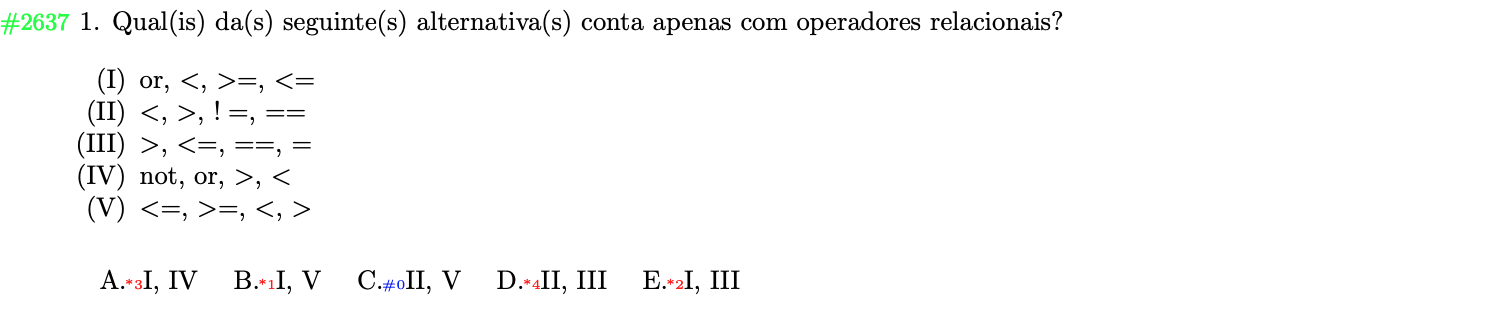
\includegraphics[width=0.9\textwidth]{ApeB_q1.png}
     \caption{Questão da taxonomia Lembrar, com chave 2637.}
  \label{fig:ApeB_q1}
\end{figure}

\begin{figure}[!ht]
    \centering
    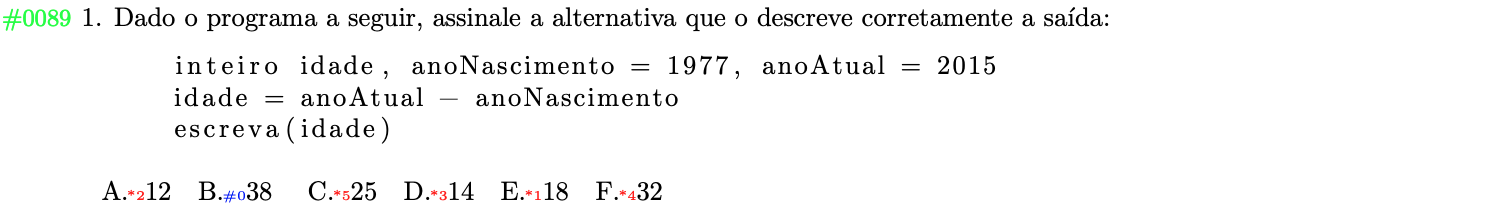
\includegraphics[width=0.9\textwidth]{ApeB_q2.png}
     \caption{Questão da taxonomia Entender (Grupo 2), com chave 89.}
  \label{fig:ApeB_q2}
\end{figure}

\begin{figure}[!ht]
    \centering
    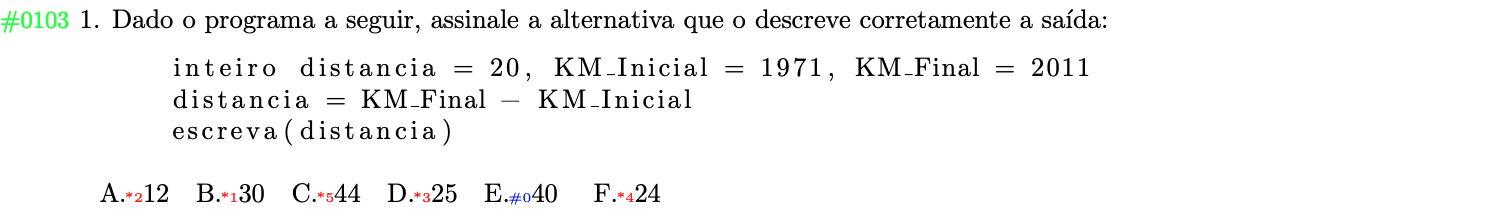
\includegraphics[width=0.9\textwidth]{ApeB_q3.png}
     \caption{Questão da taxonomia Entender (Grupo 2), com chave 103.}
  \label{fig:ApeB_q3}
\end{figure}

\begin{figure}[!ht]
    \centering
    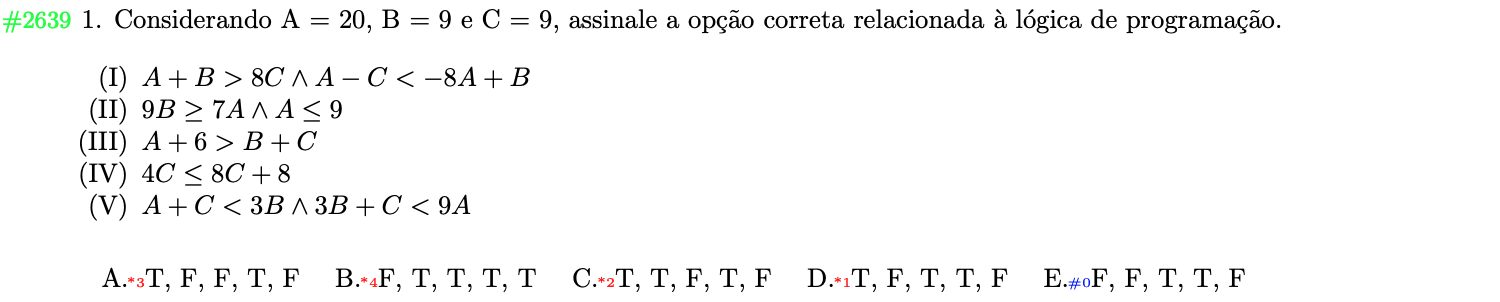
\includegraphics[width=0.9\textwidth]{ApeB_q4.png}
     \caption{Questão da taxonomia Entender (Grupo 3), com chave 2639.}
  \label{fig:ApeB_q4}
\end{figure}

\begin{figure}[!ht]
    \centering
    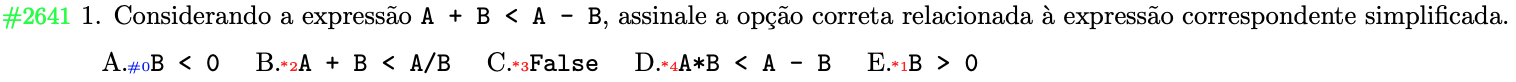
\includegraphics[width=0.9\textwidth]{ApeB_q5.png}
     \caption{Questão da taxonomia Entender (Grupo 3), com chave 2641.}
  \label{fig:ApeB_q5}
\end{figure}

\begin{figure}[!ht]
    \centering
    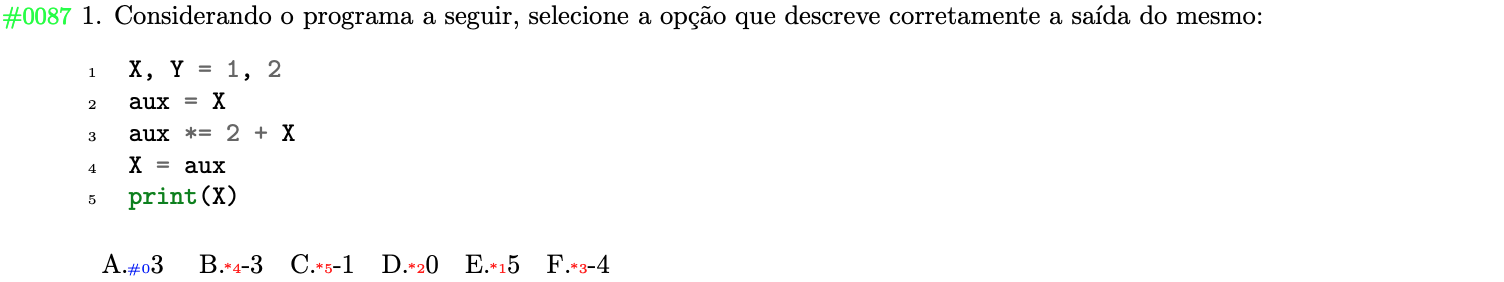
\includegraphics[width=0.9\textwidth]{ApeB_q6.png}
     \caption{Questão da taxonomia Aplicar, com chave 87.}
  \label{fig:ApeB_q6}
\end{figure}

\begin{figure}[!ht]
    \centering
    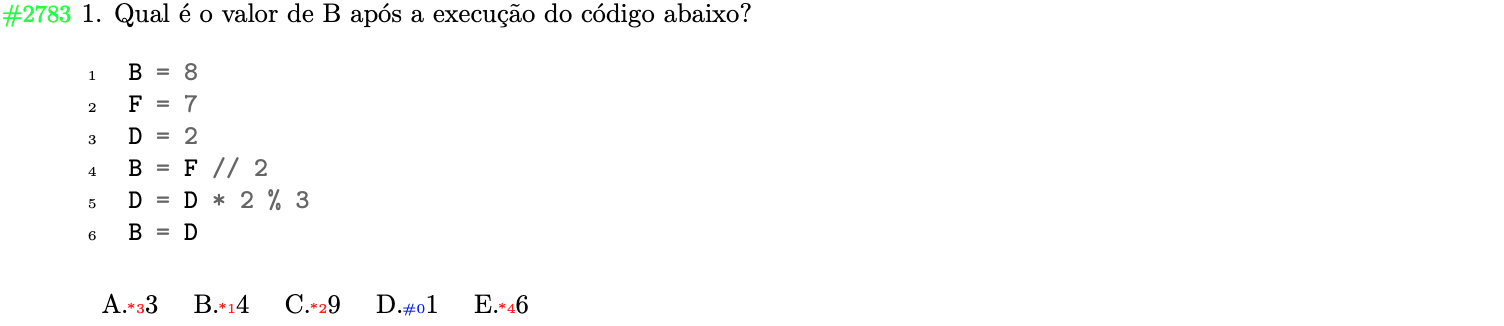
\includegraphics[width=0.9\textwidth]{ApeB_q7.png}
     \caption{Questão da taxonomia Aplicar, com chave 2783.}
  \label{fig:ApeB_q7}
\end{figure}


\section{Teste 2: Método -- SAT}

Na Seção \ref{sec:SAT_ex1} -- \nameref{sec:SAT_ex1}, o método SAT (\textit{Semi-Adaptive Testing}) foi apresentado detalhadamente por meio de um exemplo fictício. Agora, será detalhado um exemplo real de como esse método foi aplicado no curso CS1 em 2024. As identificações dos estudantes foram omitidas e, por questões de espaço, foram apresentados apenas 4 exemplos de variações do teste, bem como 4 estudantes.

Lembrando que todas as questões usadas em cada teste ainda não foram aplicadas, ou seja, ainda não existiu uma calibração baseada nas respostas dos estudantes. A única calibração foi realizada pelo professor, de forma subjetiva, classificando cada questão pelos seis níveis da Taxonomia de Bloom.

No segundo teste, abordando o tópico de método e com apenas instruções sequenciais, o teste adaptativo foi conduzido analisando os acertos dos estudantes no Teste 1, ponderado pela Taxonomia de Bloom estabelecida pelo professor.

\subsection{Criação dos testes adaptativos}

As 200 variações do Teste 2 foram ordenadas pela média das taxonomias de Bloom ($b_i$), que foram normalizadas entre -2 e 3, onde o nível Lembrar recebeu -2 e o nível Criar recebeu 3. A seguir, são apresentadas as duas variações com as menores taxonomias médias e as duas com as maiores taxonomias dentre essas 200 variações aleatórias geradas ao clicar no botão ``Criar-Variações'' na tela de exame, conforme descrito na Seção \ref{sec:adaptiveTestVariations}.

\begin{myboxCode}{corCSV}{\textbf{Arquivo \texttt{*\_adaptive\_test\_variations}}}\vspace{3mm}
    \hrule
    \begin{verbatim}
Variation  ID MeanAbilities STD  a1 a2 a3 a4 a5 b1 b2 b3 b4 b5  k1   k2   k3   k4   k5
197      75943 -1.800     0.400  1  1  1  1  1  -2 -2 -2 -1 -2 2761 2644 2728 2649 2764
 31      75777 -1.600     0.490  1  1  1  1  1  -1 -2 -1 -2 -2 2650 2710 2711 2761 2644
...
 83      75829 -0.400     0.490  1  1  1  1  1   0 -1 -1  0  0 2718 2646 2729 2715 2766
173      75919 -0.400     0.490  1  1  1  1  1  -1 -1  0  0  0 2720 2711 2766 2721 2763
\end{verbatim}
\end{myboxCode}

Na Seção \ref{sec:adaptive_test}, foram exemplificadas as habilidades anteriores de cada estudante. A seguir, são apresentadas os dois com piores e melhores habilidades. A habilidade -5 é atribuída ao estudante que faltou ao teste.

\begin{myboxCode}{corCSV}{\textbf{Arquivo \texttt{*\_adaptive\_test.csv}}}\vspace{3mm}
\hrule
\begin{verbatim}
RoomID Code Name  Email            2024-02-15:575:pi-Teste01-seq MeanPreviousAbilities
749	   A    stu01 stu01@omitido.br   -5                          -5
749	   A    stu02 stu02@omitido.br   -5                          -5
... 
749    A    stu71 stu71@omitido.br    0                           0
750    B    stu72 stu72@omitido.br    0                           0
\end{verbatim}
\end{myboxCode}

Finalmente, na Seção \ref{sec:variations}, é apresentada a variação de cada estudante. A seguir, são mostrados apenas os estudantes com as duas habilidades mais baixas e as duas mais altas. Para aumentar o número de variações atribuídas aos estudantes, foi realizado um sorteio entre as habilidades \texttt{MeanPreviousAbilities-0.05} e \texttt{MeanPreviousAbilities+0.05}, como observado na variação 173, atribuída aos dois estudantes com as melhores habilidades.

\begin{myboxCode}{corCSV}{\textbf{Arquivo \texttt{*\_variations.csv}}}\vspace{3mm}
\hrule
\begin{verbatim}
Room   Name  Email              Variation  MeanPreviousAbilities
  A    stu01 stu01@omitido.br   197        -5
  A    stu02 stu02@omitido.br   197        -5
... 
  A    stu71 stu71@omitido.br   173         0
  B    stu72 stu72@omitido.br   173         0
\end{verbatim}
\end{myboxCode}

É importante destacar que a distribuição das variações para cada estudante ocorre selecionando o estudante com a menor habilidade e atribuindo a variação com a menor média (no intervalo +/- 0.05). O mesmo procedimento é aplicado ao estudante com a maior habilidade. As demais variações são atribuídas aos estudantes de forma linear, com base em suas médias de habilidade. Para mais detalhes, consulte o método \texttt{getHashAdaptative()} no arquivo \texttt{UtilsLatex.py}\footnote{\url{https://github.com/fzampirolli/mctest/blob/master/exam/UtilsLatex.py}}.

\subsection{Correção dos testes adaptativos}

Neste segundo teste, foram registradas 58 respostas, conforme sumarizado na Tabela \ref{tab:respostas_atualizada_teste2}. As chaves das questões não estão incluídas nesta tabela, pois consistiram em 30 questões agrupadas em 14 categorias (Grupos), das quais 5 questões (uma por grupo) foram selecionadas aleatoriamente. Para todos os testes, foram geradas 200 variações. Essas questões foram adaptadas do Relatório Técnico de \citeonline{araujoestudo2020}.

É possível observar na linha de Respostas da Tabela \ref{tab:respostas_atualizada_teste2} um baixo número de respostas, devido à quantidade excessiva de questões a serem sorteadas. Isso prejudica a qualidade da calibração de cada questão. Por exemplo, a questão 14 teve apenas uma resposta correta, enquanto a questão 21 teve 15 respostas corretas, evidenciando que esta última está muito fácil e provavelmente precisa ser revisada, pois pode não estar discriminando adequadamente entre os estudantes que sabem o conteúdo e os que não sabem.

\begin{table}[!ht]
    \centering
    \caption{Porcentagem de acertos e número de questões respondidas no Teste 2: Método -- WPC.}
    \label{tab:respostas_atualizada_teste2}
    \begin{tabular}{rccccclllllllllll}
    \cline{1-10}
    \multicolumn{1}{|l|}{} & \multicolumn{9}{c|}{\cellcolor{green!25}\textbf{Lembrar}} &  &  &  &  &  &  &  \\ \cline{1-10}
    \multicolumn{1}{|r|}{\textbf{Grupos}} & \multicolumn{6}{c|}{1} & \multicolumn{1}{c|}{2} & \multicolumn{1}{c|}{3} & \multicolumn{1}{c|}{4} &  &  &  &  &  &  &  \\ \cline{1-10}
    \multicolumn{1}{|r|}{\cellcolor[HTML]{D9D9D9}\textbf{Questões}} & \multicolumn{1}{c|}{\cellcolor[HTML]{D9D9D9}1} & \multicolumn{1}{c|}{\cellcolor[HTML]{D9D9D9}2} & \multicolumn{1}{c|}{\cellcolor[HTML]{D9D9D9}3} & \multicolumn{1}{c|}{\cellcolor[HTML]{D9D9D9}4} & \multicolumn{1}{c|}{\cellcolor[HTML]{D9D9D9}5} & \multicolumn{1}{c|}{\cellcolor[HTML]{D9D9D9}6} & \multicolumn{1}{c|}{\cellcolor[HTML]{D9D9D9}7} & \multicolumn{1}{c|}{\cellcolor[HTML]{D9D9D9}8} & \multicolumn{1}{c|}{\cellcolor[HTML]{D9D9D9}9} &  &  &  &  &  &  &  \\ 
    \multicolumn{1}{|r|}{\textbf{Repostas}} & \multicolumn{1}{c|}{3} & \multicolumn{1}{c|}{5} & \multicolumn{1}{c|}{4} & \multicolumn{1}{c|}{4} & \multicolumn{1}{c|}{22} & \multicolumn{1}{c|}{7} & \multicolumn{1}{c|}{20} & \multicolumn{1}{c|}{18} & \multicolumn{1}{c|}{11} &  &  &  &  &  &  &  \\ 
    \multicolumn{1}{|r|}{\cellcolor[HTML]{D9D9D9}\textbf{Acertos \%}} & \multicolumn{1}{c|}{\cellcolor[HTML]{D9D9D9}0} & \multicolumn{1}{c|}{\cellcolor[HTML]{D9D9D9}20} & \multicolumn{1}{c|}{\cellcolor[HTML]{D9D9D9}75} & \multicolumn{1}{c|}{\cellcolor[HTML]{D9D9D9}0} & \multicolumn{1}{c|}{\cellcolor[HTML]{D9D9D9}9} & \multicolumn{1}{c|}{\cellcolor[HTML]{D9D9D9}43} & \multicolumn{1}{c|}{\cellcolor[HTML]{D9D9D9}30} & \multicolumn{1}{c|}{\cellcolor[HTML]{D9D9D9}83} & \multicolumn{1}{c|}{\cellcolor[HTML]{D9D9D9}36} &  &  &  &  &  &  &  \\ \cline{1-10}
    \multicolumn{1}{l}{} & \multicolumn{1}{l}{} & \multicolumn{1}{l}{} & \multicolumn{1}{l}{} & \multicolumn{1}{l}{} & \multicolumn{1}{l}{} &  &  &  &  &  &  &  &  &  &  &  \\ \hline
    \multicolumn{1}{|l|}{} & \multicolumn{16}{c|}{\cellcolor{yellow!25}\textbf{Entender}} \\ \hline
    \multicolumn{1}{|r|}{\textbf{Grupos}} & \multicolumn{1}{c|}{5} & \multicolumn{10}{c|}{6} & \multicolumn{3}{c|}{7} & \multicolumn{1}{c|}{8} & \multicolumn{1}{c|}{9} \\ \hline
    \rowcolor[HTML]{D9D9D9} 
    \multicolumn{1}{|r|}{\cellcolor[HTML]{D9D9D9}\textbf{Questões}} & \multicolumn{1}{c|}{\cellcolor[HTML]{D9D9D9}10} & \multicolumn{1}{c|}{\cellcolor[HTML]{D9D9D9}11} & \multicolumn{1}{c|}{\cellcolor[HTML]{D9D9D9}12} & \multicolumn{1}{c|}{\cellcolor[HTML]{D9D9D9}13} & \multicolumn{1}{c|}{\cellcolor[HTML]{D9D9D9}14} & \multicolumn{1}{c|}{\cellcolor[HTML]{D9D9D9}15} & \multicolumn{1}{c|}{\cellcolor[HTML]{D9D9D9}16} & \multicolumn{1}{c|}{\cellcolor[HTML]{D9D9D9}17} & \multicolumn{1}{c|}{\cellcolor[HTML]{D9D9D9}18} & \multicolumn{1}{c|}{\cellcolor[HTML]{D9D9D9}19} & \multicolumn{1}{c|}{\cellcolor[HTML]{D9D9D9}20} & \multicolumn{1}{c|}{\cellcolor[HTML]{D9D9D9}21} & \multicolumn{1}{c|}{\cellcolor[HTML]{D9D9D9}22} & \multicolumn{1}{c|}{\cellcolor[HTML]{D9D9D9}23} & \multicolumn{1}{c|}{\cellcolor[HTML]{D9D9D9}24} & \multicolumn{1}{c|}{\cellcolor[HTML]{D9D9D9}25} \\ 
    \multicolumn{1}{|r|}{\textbf{Repostas}} & \multicolumn{1}{c|}{8} & \multicolumn{1}{c|}{3} & \multicolumn{1}{c|}{2} & \multicolumn{1}{c|}{18} & \multicolumn{1}{c|}{1} & \multicolumn{1}{c|}{1} & \multicolumn{1}{c|}{2} & \multicolumn{1}{c|}{8} & \multicolumn{1}{c|}{3} & \multicolumn{1}{c|}{12} & \multicolumn{1}{c|}{6} & \multicolumn{1}{c|}{15} & \multicolumn{1}{c|}{8} & \multicolumn{1}{c|}{18} & \multicolumn{1}{c|}{8} & \multicolumn{1}{c|}{3} \\ 
    \rowcolor[HTML]{D9D9D9} 
    \multicolumn{1}{|r|}{\cellcolor[HTML]{D9D9D9}\textbf{Acertos \%}} & \multicolumn{1}{c|}{\cellcolor[HTML]{D9D9D9}50} & \multicolumn{1}{c|}{\cellcolor[HTML]{D9D9D9}67} & \multicolumn{1}{c|}{\cellcolor[HTML]{D9D9D9}50} & \multicolumn{1}{c|}{\cellcolor[HTML]{D9D9D9}39} & \multicolumn{1}{c|}{\cellcolor[HTML]{D9D9D9}100} & \multicolumn{1}{c|}{\cellcolor[HTML]{D9D9D9}0} & \multicolumn{1}{c|}{\cellcolor[HTML]{D9D9D9}50} & \multicolumn{1}{c|}{\cellcolor[HTML]{D9D9D9}100} & \multicolumn{1}{c|}{\cellcolor[HTML]{D9D9D9}0} & \multicolumn{1}{c|}{\cellcolor[HTML]{D9D9D9}33} & \multicolumn{1}{c|}{\cellcolor[HTML]{D9D9D9}50} & \multicolumn{1}{c|}{\cellcolor[HTML]{D9D9D9}100} & \multicolumn{1}{c|}{\cellcolor[HTML]{D9D9D9}50} & \multicolumn{1}{c|}{\cellcolor[HTML]{D9D9D9}56} & \multicolumn{1}{c|}{\cellcolor[HTML]{D9D9D9}63} & \multicolumn{1}{c|}{\cellcolor[HTML]{D9D9D9}100} \\ \hline
    \multicolumn{1}{l}{} & \multicolumn{1}{l}{} & \multicolumn{1}{l}{} & \multicolumn{1}{l}{} & \multicolumn{1}{l}{} & \multicolumn{1}{l}{} &  &  &  &  &  &  &  &  &  &  &  \\ \cline{1-6}
    \multicolumn{1}{|l|}{} & \multicolumn{5}{c|}{\cellcolor{red!25}\textbf{Aplicar}} &  &  &  &  &  &  &  &  &  &  &  \\ \cline{1-6}
    \multicolumn{1}{|r|}{\textbf{Grupos}} & \multicolumn{1}{c|}{10} & \multicolumn{1}{c|}{11} & \multicolumn{1}{c|}{12} & \multicolumn{1}{c|}{13} & \multicolumn{1}{c|}{14} &  &  &  &  &  &  &  &  &  &  &  \\ \cline{1-6}
    \multicolumn{1}{|r|}{\cellcolor[HTML]{D9D9D9}\textbf{Questões}} & \multicolumn{1}{c|}{\cellcolor[HTML]{D9D9D9}26} & \multicolumn{1}{c|}{\cellcolor[HTML]{D9D9D9}27} & \multicolumn{1}{c|}{\cellcolor[HTML]{D9D9D9}28} & \multicolumn{1}{c|}{\cellcolor[HTML]{D9D9D9}29} & \multicolumn{1}{c|}{\cellcolor[HTML]{D9D9D9}30} &  &  &  &  &  &  &  &  &  &  &  \\ 
    \multicolumn{1}{|r|}{\textbf{Repostas}} & \multicolumn{1}{c|}{13} & \multicolumn{1}{c|}{7} & \multicolumn{1}{c|}{24} & \multicolumn{1}{c|}{17} & \multicolumn{1}{c|}{19} &  &  &  &  &  &  &  &  &  &  &  \\ 
    \multicolumn{1}{|r|}{\cellcolor[HTML]{D9D9D9}\textbf{Acertos \%}} & \multicolumn{1}{c|}{\cellcolor[HTML]{D9D9D9}31} & \multicolumn{1}{c|}{\cellcolor[HTML]{D9D9D9}29} & \multicolumn{1}{c|}{\cellcolor[HTML]{D9D9D9}46} & \multicolumn{1}{c|}{\cellcolor[HTML]{D9D9D9}41} & \multicolumn{1}{c|}{\cellcolor[HTML]{D9D9D9}58} &  &  &  &  &  &  &  &  &  &  &  \\ \cline{1-6}
    \multicolumn{5}{r}{\cellcolor[HTML]{F9CB9C}\textbf{média de acertos \%}} & \multicolumn{1}{c}{\cellcolor[HTML]{F9CB9C}47} \\ 
    \multicolumn{5}{r}{\cellcolor[HTML]{F9CB9C}\textbf{desvio padrão}} & \multicolumn{1}{c}{\cellcolor[HTML]{F9CB9C}30} \\ 
    \end{tabular}
    \end{table}


\section{Teste 3: Condicional -- WPC}

O Teste 3 sobre questões envolvendo condicionais utiliza o método \textit{Weighted Probability of Correctness} (WPC) ou Porcentagem Ponderada de Acertos para avaliar as habilidades dos estudantes e será detalhado a seguir sua utilização nas duas turmas.

\subsection{Criação dos testes adaptativos}

Como as 18 questões usadas neste teste são novas, a Taxonomia de Bloom também é considerada para definir os pesos das variações. O arquivo \texttt{*\_adaptive\_test\_variations.csv} é similar em todos os 5 testes adaptativos aplicados. No arquivo \texttt{*\_adaptive\_test.csv} gerado ao clicar em ``Criar-PDF'', é considerada a porcentagem de acerto de cada questão, multiplicada por 1 se o estudante acertou ou 0 caso contrário. Esses valores são somados e então normalizados entre -5 e 5. As primeiras colunas com identificação da turma e do estudante foram omitidas a seguir. As questões foram adaptadas do Relatório Técnico de \citeonline{araujoestudo2020}.

\begin{myboxCode}{corCSV}{\textbf{Arquivo \texttt{*\_adaptive\_test.csv}}}\vspace{3mm}
\hrule
\begin{verbatim}
... 2024-2-15:575:pi-Teste01-seq 2024-2-22:576:pi-Teste02-método MeanPreviousAbilities
...          -5                            -5                           -5
...          -5                            -5                           -5
... 
...           2.092                         2.158                        2.125
...           2.128                         2.325                        2.226
\end{verbatim}
\end{myboxCode}

\subsection{Correção dos testes adaptativos}

A Tabela \ref{tab:respostas_atualizada_teste3} apresenta a porcentagem de acertos e o número de questões respondidas no Teste 3, agrupadas de acordo com a Taxonomia de Bloom. Cada coluna representa uma categoria da taxonomia. Os grupos numerados de 1 a 6 indicam os grupos de questões, lembrando que são sorteadas 5 questões em cada teste e uma questão por grupo. Neste teste, foram 56 respondentes. O número de respostas indica quantos estudantes responderam a cada questão, enquanto a porcentagem de acertos reflete a taxa de sucesso dos estudantes ao responderem cada questão.

\begin{table}[!ht]
    \centering
    \caption{Porcentagem de acertos e número de questões respondidas no Teste 3: Condicional -- WPC.}
    \label{tab:respostas_atualizada_teste3}
    \setlength{\tabcolsep}{4.2pt} % Reduzindo o espaçamento entre as colunas
    \begin{tabular}{|r|*{18}{c|}}
        \hline
        \multicolumn{1}{|l|}{} & \multicolumn{2}{c|}{\cellcolor{green!25}\textbf{Lembrar}} & \multicolumn{4}{c|}{\cellcolor{yellow!25}\textbf{Entender}} & \multicolumn{6}{|c|}{\cellcolor{red!25}\textbf{Aplicar}} & \multicolumn{2}{c|}{\cellcolor{blue!25}\textbf{Analisar}} & \multicolumn{2}{c|}{\cellcolor[HTML]{FFE599}\textbf{Avaliar}} & \multicolumn{2}{c|}{\cellcolor[HTML]{D5A6BD}\textbf{Criar}} \\ \hline
        \textbf{Grupos} & \multicolumn{2}{c|}{1} & \multicolumn{4}{c|}{2} & \multicolumn{6}{c|}{3} & \multicolumn{2}{c|}{4} & \multicolumn{2}{c|}{5} & \multicolumn{2}{c|}{6} \\\hline
        \rowcolor[HTML]{D9D9D9} 
        \textbf{Questões} & \ \ 1 \ \ & 2 & 3 & 4 & 5 & 6 & 7 & 8 & 9 & 10 & 11 & 12 & \ 13 \ & 14 & \ 15 \ & 16 & 17 & 18 \\
        \textbf{Respostas} & 17 & 23 & 9 & 15 & 11 & 17 & 8 & 10 & 12 & 10 & 4 & 12 & 14 & 29 & 26 & 20 & 26 & 17 \\ \rowcolor[HTML]{D9D9D9} 
        \textbf{Acertos \%} & 94 & 30 & 78 & 87 & 73 & 94 & 88 & 90 & 58 & 100 & 100 & 25 & 50 & 72 & 81 & 20 & 31 & 65 \\ \hline
        \multicolumn{13}{r}{} & \multicolumn{5}{r}{\cellcolor[HTML]{F9CB9C}\textbf{média de acertos \%}} & \multicolumn{1}{c}{\cellcolor[HTML]{F9CB9C}69} \\ 
        \multicolumn{13}{r}{} & \multicolumn{5}{r}{\cellcolor[HTML]{F9CB9C}\textbf{desvio padrão}} & \multicolumn{1}{c}{\cellcolor[HTML]{F9CB9C}26} \\ 
    \end{tabular}
\end{table}

\section{Teste 4: Repetição -- WPC}

O Teste 4, centrado em questões relacionadas à repetição, também utiliza o método de avaliação WPC (\textit{Weighted Probability of Correctness}) para determinar as habilidades dos estudantes, seguindo uma abordagem semelhante à apresentada na seção anterior. Nesta seção, são apresentados exclusivamente os resultados da correção deste teste aplicado às duas turmas. A Tabela \ref{tab:respostas_atualizada_teste4} não inclui uma linha de grupos devido à ausência de grupos com mais de uma questão. Assim, cada questão é tratada como um grupo individual e possui a mesma probabilidade de ser selecionada entre as 5 questões do teste. Nesta aplicação, houve um total de 50 respondentes.

\begin{table}[!ht]
    \centering
    \caption{Porcentagem de acertos e número de questões respondidas no Teste 4: Repetição -- WPC.}
    \label{tab:respostas_atualizada_teste4}
    \begin{tabular}{|r|*{16}{c|}}
        \hline
        \multicolumn{1}{|l|}{} & \multicolumn{8}{c|}{\cellcolor{green!25}\textbf{Lembrar}} & \multicolumn{4}{c|}{\cellcolor{yellow!25}\textbf{Entender}} & \multicolumn{4}{c|}{\cellcolor{red!25}\textbf{Aplicar}} \\\hline
        \rowcolor[HTML]{D9D9D9} 
        \textbf{Questões}    & 1  & 2 & 3 & 4 & 5 & 6 & 7 & 8 & 9 & 10 & 11 & 12 & 13 & 14 & 15 & 16 \\
        \textbf{Repostas}   & 10 & 14 & 4 & 9 & 11 & 11 & 10 & 14 & 6 & 11 & 10 & 10 & 9 & 13 & 17 & 11 \\
        \rowcolor[HTML]{D9D9D9} 
        \textbf{Acertos \%} & 30 & 57 & 100 & 89 & 64 & 64 & 60 & 50 & 33 & 55 & 60 & 10 & 22 & 23 & 71 & 55 \\ \hline
        \multicolumn{11}{r}{} & \multicolumn{5}{r}{\cellcolor[HTML]{F9CB9C}\textbf{média de acertos \%}} & \multicolumn{1}{c}{\cellcolor[HTML]{F9CB9C}53} \\ 
        \multicolumn{11}{r}{} & \multicolumn{5}{r}{\cellcolor[HTML]{F9CB9C}\textbf{desvio padrão}} & \multicolumn{1}{c}{\cellcolor[HTML]{F9CB9C}23} \\ 
    \end{tabular}
\end{table}

\section{Teste 5: Vetor -- MLE-v0}

O Teste 5, que trata de vetores, utiliza o teste adaptativo MLE (\textit{Maximum Likelihood Estimation}) em sua primeira versão. Nesse método, a média do produto da habilidade da questão \( b_i \) é calculada, sendo multiplicada por 1 se o estudante acertou a questão ou 0 caso contrário. Essa abordagem segue os mesmos princípios aplicados nos tipos SAT e WPC, conforme demonstrado anteriormente. Neles, a habilidade média do estudante nos quatro testes anteriores é usada para determinar variações proporcionais à dificuldade das variações, considerando uma distribuição linear. Por exemplo, o estudante com menor habilidade média recebe uma variação com a menor média dos \( b_i \), e assim por diante. Na próxima seção, será feita uma comparação com a forma clássica de \textit{Test Information} \cite{baker2017basics}.

A Tabela \ref{tab:respostas_atualizada_teste5} exibe a porcentagem de acertos e o número de questões respondidas no Teste 5, agrupadas por Taxonomia de Bloom. As questões estão distribuídas entre as categorias Lembrar, Entender, Aplicar e Analisar. As colunas correspondem às diferentes categorias de Bloom e as respectivas questões. Os valores de Repostas indicam o número de respostas para cada questão, e os valores de Acertos mostram a porcentagem de acertos para cada questão. Neste teste foram 53 respondentes.


\begin{table}[!ht]
    \centering
    \caption{Porcentagem de acertos e número de questões respondidas no Teste 5: Vetor -- MLE.}
    \label{tab:respostas_atualizada_teste5}
    \setlength{\tabcolsep}{4.7pt} % Reduzindo o espaçamento entre as colunas
    \begin{tabular}{|r|*{18}{c|}}
        \hline
        \multicolumn{1}{|l|}{} & \multicolumn{3}{c|}{\cellcolor{green!25}\textbf{Lembrar}} & \multicolumn{4}{c|}{\cellcolor{yellow!25}\textbf{Entender}} & \multicolumn{9}{c|}{\cellcolor{red!25}\textbf{Aplicar}} & \multicolumn{2}{c|}{\cellcolor{blue!25}\textbf{Analisar}} \\ \hline
        \rowcolor[HTML]{D9D9D9} 
        \textbf{Questões} & 1 & 2 & 3 & 4 & 5 & 6 & 7 & 8 & 9 & 10 & 11 & 12 & 13 & 14 & 15 & 16 & \  17 \ & \  18 \   \\
        \textbf{Repostas} & 8 & 22 & 31 & 32 & 16 & 9 & 8 & 25 & 9 & 27 & 13 & 13 & 12 & 11 & 5 & 6 & 9 & 9 \\
        \rowcolor[HTML]{D9D9D9} 
        \textbf{Acertos \%} & 50 & 73 & 35 & 41 & 44 & 33 & 50 & 24 & 56 & 33 & 54 & 54 & 67 & 27 & 0 & 67 & 33 & 11 \\ \hline
        \multicolumn{13}{r}{} & \multicolumn{5}{r}{\cellcolor[HTML]{F9CB9C}\textbf{média de acertos \%}} & \multicolumn{1}{c}{\cellcolor[HTML]{F9CB9C}42} \\ 
        \multicolumn{13}{r}{} & \multicolumn{5}{r}{\cellcolor[HTML]{F9CB9C}\textbf{desvio padrão}} & \multicolumn{1}{c}{\cellcolor[HTML]{F9CB9C}19} \\ 
    \end{tabular}
\end{table}


\section{Teste 6: Matriz -- MLE-v1}

No Teste 6, que aborda matrizes, foi empregado uma segunda versão do método adaptativo MLE (\textit{Maximum Likelihood Estimation}). Nessa abordagem, o conceito de \textit{Test Information} (TI) foi utilizado para atribuir a melhor variação ao estudante. 

A Tabela \ref{tab:respostas_atualizada_teste6} apresenta a porcentagem de acertos e o número de questões respondidas no Teste 6, agrupadas por Taxonomia de Bloom. As respostas estão distribuídas em três categorias: Lembrar, Entender e Aplicar. Cada categoria abrange um conjunto específico de chaves de questão, com seus respectivos números de respostas e percentuais de acertos. Vale ressaltar que, devido ao número limitado de variações atribuídas aos estudantes, as questões com as chaves 3077 e 268 não foram sorteadas. Foram 55 respondentes neste Teste 6.

Para obter mais detalhes sobre as correções realizadas e o método utilizado, é possível consultar a função \texttt{getHashVariationByCat()} no arquivo \texttt{UtilsLatex.py}, disponível no GitHub\footnote{\url{https://github.com/fzampirolli/mctest/blob/master/exam/UtilsLatex.py}.}. Atualmente, em caso de empate nos valores de TI, uma variação é selecionada aleatoriamente dentro do intervalo +/- 0.05 do valor de TI.

\begin{table}[!ht]
\centering
\caption{Porcentagem de acertos e número de questões respondidas no Teste 6: Matriz -- MLE.}
\label{tab:respostas_atualizada_teste6}
\begin{tabular}{|r|*{11}{c|}}
    \hline
    & \multicolumn{3}{c|}{\cellcolor[HTML]{B6D7A8}\textbf{Lembrar}} & \multicolumn{5}{c|}{\cellcolor[HTML]{FFFF00}\textbf{Entender}} & \multicolumn{3}{c|}{\cellcolor[HTML]{F4CCCC}\textbf{Aplicar}} \\  \hline
\rowcolor[HTML]{D9D9D9} 
\multicolumn{1}{|r|}{\cellcolor[HTML]{D9D9D9}\textbf{Chaves}} & 
264	& 3078 & 3079 & 3077 & 3081 & 3083 & 3084 & 3085 & 268 & 3086 & 3087 \\ 
\multicolumn{1}{|r|}{\textbf{Repostas}} & 43 & 47 & 50 &   & 16 & 9 & 5 & 44 &   & 46 & 15 \\
\rowcolor[HTML]{D9D9D9} 
\textbf{Acertos \%} & 93 & 85 & 34 &  & 31 & 33 & 60 & 43 &  & 48 & 60 \\ \hline
\multicolumn{7}{r}{} & \multicolumn{4}{r}{\cellcolor[HTML]{F9CB9C}\textbf{média de acertos \%}} & \multicolumn{1}{c}{\cellcolor[HTML]{F9CB9C}54} \\ 
\multicolumn{7}{r}{} & \multicolumn{4}{r}{\cellcolor[HTML]{F9CB9C}\textbf{desvio padrão}} & \multicolumn{1}{c}{\cellcolor[HTML]{F9CB9C}21} \\ 
\end{tabular}
\end{table}


A fim de aumentar a variedade de variações sorteadas (na Tabela \ref{tab:MLE_frequencias}, versão 0, sempre foi atribuída a primeira variação com o mesmo TI), porém, agora quando ocorre um empate no TI, é selecionada aleatoriamente uma variação dentro de um intervalo de TI, conforme mencionado anteriormente. Como mostrado na Tabela \ref{tab:MLE_frequencias}, no primeiro caso foram geradas 6 variações e no segundo caso 15 variações. Em comparação com o método WPC aplicado ao Teste 6, foram utilizadas 54 variações distintas distribuídas linearmente entre os estudantes. Nas duas turmas foram 72 estudantes matriculados. Ou seja, a probabilidade de dois estudantes receberem a mesma variação e sentarem próximos é baixa na correção do MLE-v1 e também nos métodos adaptativos WPC e SAT.

\begin{table}[!ht]
    \centering
    \caption{Comparação entre as frequências das variações.}
    \label{tab:MLE_frequencias}
    \rowcolors{2}{gray!25}{white}
    \begin{tabular}{|c|c|c|c|}
        \hline
        \cellcolor{green!25} \textbf{Versão 0} & \cellcolor{green!25} \textbf{Frequência} & \cellcolor{yellow!25} \textbf{Versão 1} & \cellcolor{yellow!25} \textbf{Frequência} \\
        \hline
        8 & 2 & 21 & 1 \\
        15 & 1 & 24 & 1 \\
        37 & 54 & 37 & 5 \\
        81 & 8 & 44 & 13 \\
        193 & 6 & 65 & 2 \\
        199 & 3 & 81 & 4 \\
        & & 108 & 5 \\
        & & 121 & 6 \\
        & & 179 & 1 \\
        & & 184 & 14 \\
        & & 186 & 1 \\
        & & 188 & 4 \\
        & & 193 & 1 \\
        & & 194 & 4 \\
        & & 199 & 12 \\
        \hline
    \end{tabular}
\end{table}

\subsection{Descrição das questões utilizadas}\label{sec:questoesTeste6}

Esta seção apresenta uma descrição das questões utilizadas no Teste 6, organizadas de acordo com a Taxonomia de Bloom. As Figuras \ref{fig:ApeB_0264}, \ref{fig:ApeB_3078} e \ref{fig:ApeB_3079} correspondem a questões da taxonomia Lembrar, com chaves 264, 3078 e 3079, respectivamente. Já as Figuras \ref{fig:ApeB_3081}, \ref{fig:ApeB_3083}, \ref{fig:ApeB_3084} e \ref{fig:ApeB_3085} representam questões da taxonomia Entender, com chaves 3081, 3083, 3084 e 3085, respectivamente. Por fim, as Figuras \ref{fig:ApeB_3086} e \ref{fig:ApeB_3087} correspondem a questões da taxonomia Aplicar, com chaves 3086 e 3087, respectivamente. Cada figura apresenta o enunciado da questão, a sua respectiva chave e as alternativas, onde o destaque em azul representa a alternativa correta (marcada como \#0). 

Diferentemente das provas avaliativas, essas questões são simples e devem ser respondidas em até 30 minutos. Mesmo assim, é possível observar, exceto nas duas primeiras questões, que muitos estudantes erram as respostas, o que pode indicar uma falta de dedicação aos estudos, conforme também apontado no Apêndice \ref{ch:apendice} -- \nameref{ch:apendice}. Vale lembrar que as questões utilizadas nos testes foram aplicadas pela primeira vez e melhorias deverão ser realizadas, analisando, por exemplo, a Curva Característica do Item. Além disso, a questão com chave 3078 está mal formulada, pois não existe estrutura de dados matriz em Python, mas sim lista (no curso CS1 não foi abordado bibliotecas, como Numpy).

\begin{figure}[!ht]
    \centering
    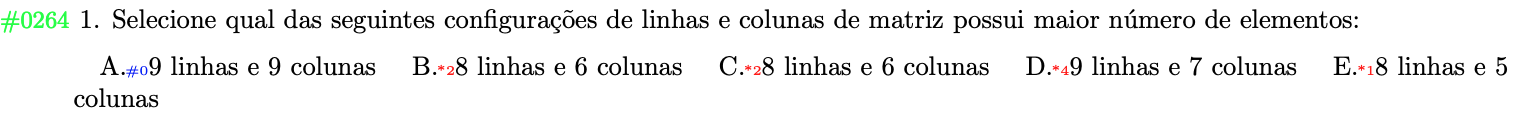
\includegraphics[width=0.9\textwidth]{ApeB_0264.png}
     \caption{Questão da taxonomia Lembrar, com chave 264.}
  \label{fig:ApeB_0264}
\end{figure}

\begin{figure}[!ht]
    \centering
    
\includegraphics[width=0.9\textwidth]{ApeB_3078.png}
     \caption{Questão da taxonomia Lembrar, com chave 3078.}
  \label{fig:ApeB_3078}
\end{figure}

\begin{figure}[!ht]
    \centering
    
\includegraphics[width=0.9\textwidth]{ApeB_3079.png}
     \caption{Questão da taxonomia Lembrar, com chave 3079.}
  \label{fig:ApeB_3079}
\end{figure}

\begin{figure}[!ht]
    \centering
    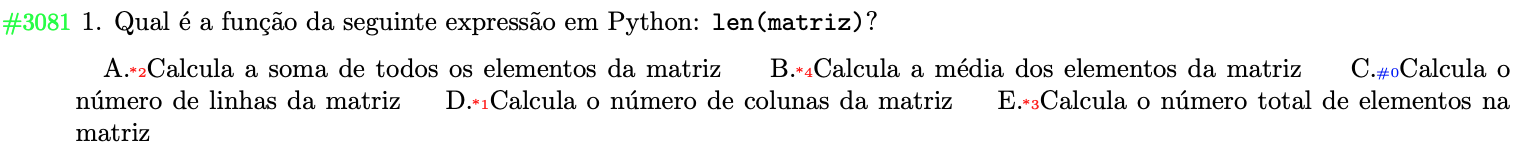
\includegraphics[width=0.9\textwidth]{ApeB_3081.png}
     \caption{Questão da taxonomia Entender, com chave 3081.}
  \label{fig:ApeB_3081}
\end{figure}

\begin{figure}[!ht]
    \centering
    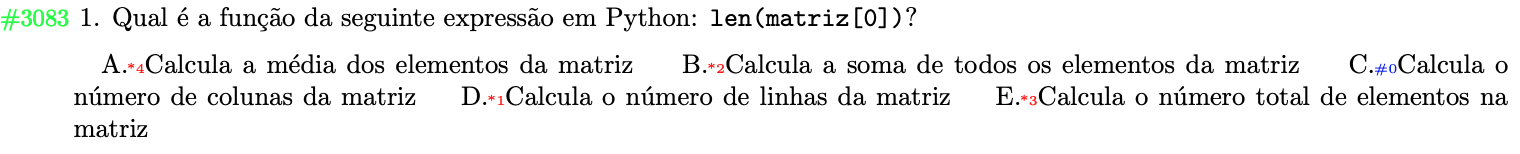
\includegraphics[width=0.9\textwidth]{ApeB_3083.png}
     \caption{Questão da taxonomia Entender, com chave 3083.}
  \label{fig:ApeB_3083}
\end{figure}

\begin{figure}[!ht]
    \centering
    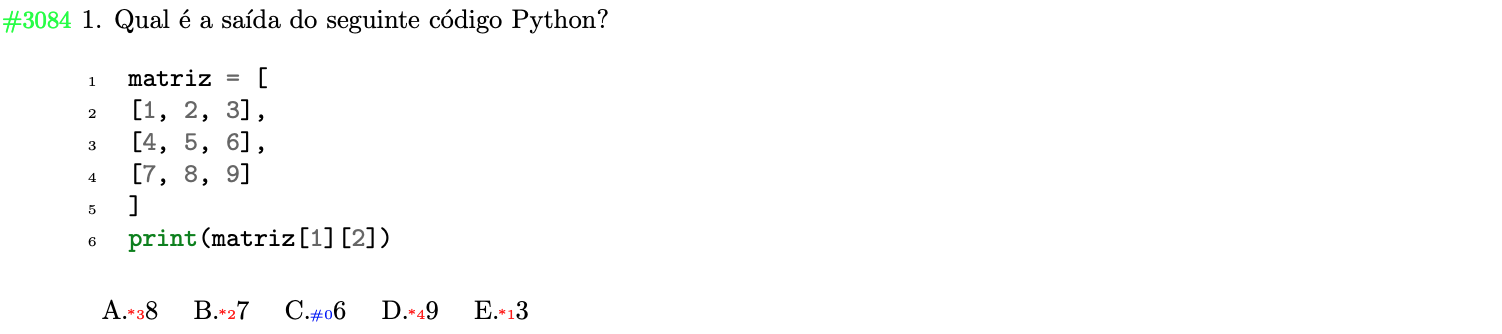
\includegraphics[width=0.9\textwidth]{ApeB_3084.png}
     \caption{Questão da taxonomia Entender, com chave 3084.}
  \label{fig:ApeB_3084}
\end{figure}

\begin{figure}[!ht]
    \centering
    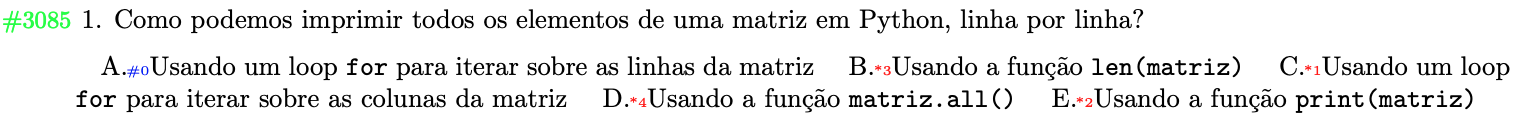
\includegraphics[width=0.9\textwidth]{ApeB_3085.png}
     \caption{Questão da taxonomia Entender, com chave 3085.}
  \label{fig:ApeB_3085}
\end{figure}

\begin{figure}[!ht]
    \centering
    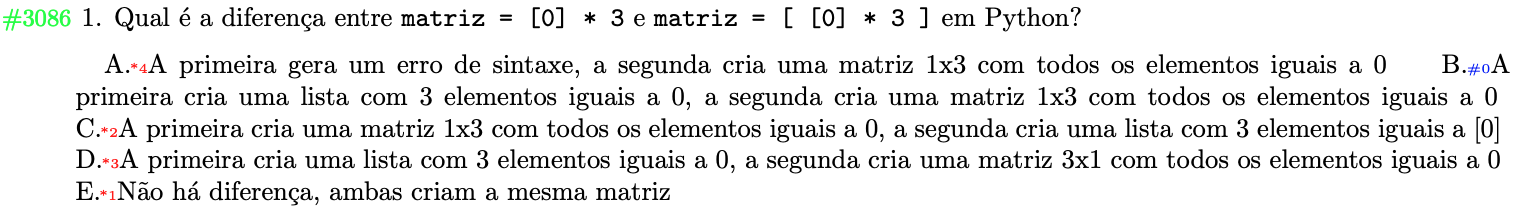
\includegraphics[width=0.9\textwidth]{ApeB_3086.png}
     \caption{Questão da taxonomia Aplicar, com chave 3086.}
  \label{fig:ApeB_3086}
\end{figure}

\begin{figure}[!ht]
    \centering
    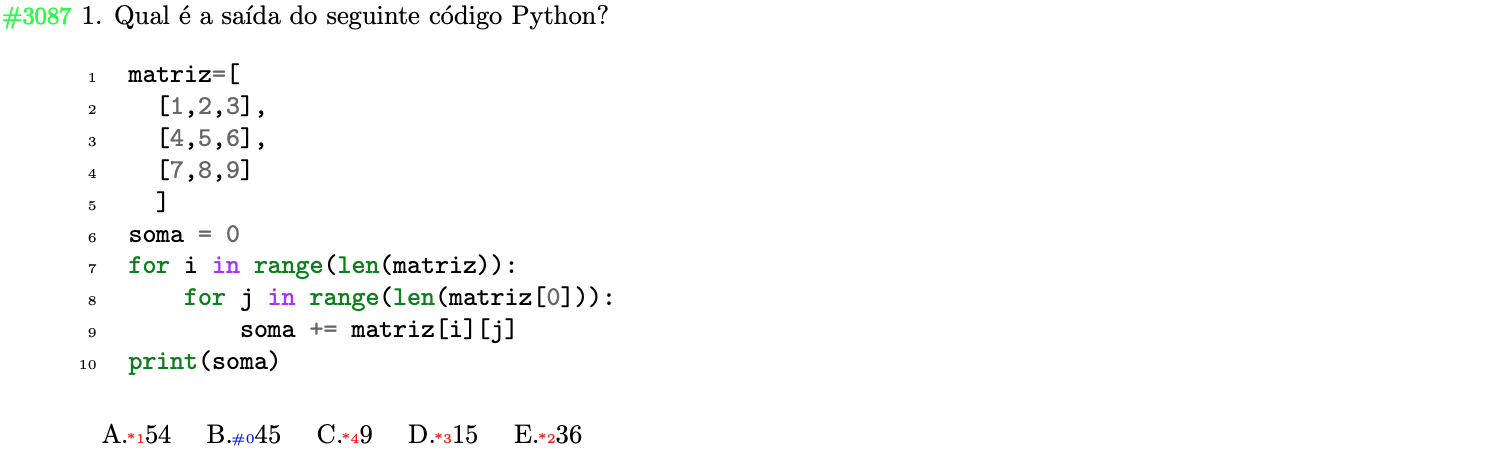
\includegraphics[width=0.9\textwidth]{ApeB_3087.png}
     \caption{Questão da taxonomia Aplicar, com chave 3087.}
  \label{fig:ApeB_3087}
\end{figure}

\subsection{Calibração das questões}\label{sec:calibracao}

A estimativa dos parâmetros da Teoria de Resposta ao Item (TRI), ou calibração, foi introduzida na Seção \ref{sec:estimativas_TRI} -- \nameref{sec:estimativas_TRI}, utilizando o método \verb|minimize| da biblioteca \verb|scipy.optimize|. Essa abordagem foi adotada devido à conveniência de ter o MCTest implementado em Python. Entretanto, nesta seção, serão apresentadas análises utilizando a linguagem R, pois essa possui diversos recursos gráficos que facilitam a visualização e interpretação dos resultados.

A Tabela \ref{tab:parameters} contém os parâmetros obtidos a partir da calibração dos itens utilizando diferentes modelos de ajuste. Os modelos foram ajustados aos dados empregando a função \verb|mirt()| do pacote R chamado \verb|mirt|.

O modelo de 1 parâmetro (1PL) foi ajustado aos dados, utilizando o modelo de Rasch. Os parâmetros estimados para cada item no modelo 1PL são apresentados na coluna 1PL da tabela.

Em seguida, o modelo de 2 parâmetros (2PL) foi ajustado aos dados. Esse modelo leva em consideração tanto a habilidade dos participantes quanto a dificuldade dos itens. Os parâmetros estimados para cada item no modelo 2PL são apresentados nas colunas 2PL da tabela, com os valores correspondentes para os parâmetros de discriminação (representados por $a$) e dificuldade (representados por $b$).

Por fim, o modelo de 3 parâmetros (3PL) foi ajustado aos dados. Esse modelo considera a habilidade dos participantes, a dificuldade dos itens e a chance de acerto ao acaso. Os parâmetros estimados para cada item no modelo 3PL são apresentados nas colunas 3PL da tabela, com os valores correspondentes para os parâmetros de discriminação (representados por $a$), dificuldade (representados por $b$) e chance de acerto ao acaso (representados por $c$).

Alguns pontos importantes a destacar nesta tabela:
\begin{itemize}
    \item Nos modelos 2PL e 3PL, os valores de dificuldade (parâmetro $b$) encontram-se fora do intervalo recomendado de -5 a 5 implementado no MCTest. Isso indica que alguns itens podem estar muito fáceis ou muito difíceis para a população avaliada;
    \item Os valores de discriminação (parâmetro $a$) também não se encontram dentro do intervalo ideal de 0,5 a 1,5. Estes valores foram estimados empiricamente após alguns testes no Colab\footnote{\url{https://colab.research.google.com/drive/1ka7_SR_QB4G7ZPVvH3p_E0bZEbOH1vhK}.}. Alguns itens apresentam baixa capacidade de discriminar entre indivíduos com diferentes níveis de proficiência;
    \item Essa falta de adequação dos parâmetros aos intervalos esperados sugere que as questões não foram bem calibradas, provavelmente devido ao baixo número de respondentes utilizado nessa análise inicial.
\end{itemize}
Portanto, serão necessários ajustes adicionais no futuro, como coletar mais dados e refinar o processo de calibração dos itens, para melhorar a qualidade psicométrica desses instrumentos. Apenas dessa forma será possível obter uma avaliação mais confiável do construto de interesse.

\begin{table}[!ht]
    \centering
\caption{Parâmetros da TRI nos Modelos 1PL, 2PL e 3PL, Além de Média e Desvio Padrão.}
    \label{tab:parameters}\normalsize
    \begin{tabular}{cccccccccc}
    \toprule
    & & \multicolumn{1}{c}{1PL} & \multicolumn{2}{c}{2PL} & \multicolumn{3}{c}{3PL} & \multicolumn{2}{c}{Estatísticas} \\
    \cmidrule(r){3-3} \cmidrule(r){4-5} \cmidrule(r){6-8} \cmidrule(r){9-10}
    & Chaves & $b$ & $a$ & $b$ & $a$ & $b$ & $c$ & Média & DP \\
    \midrule
    \cellcolor{green!25}\textbf{Lembrar} & 264 & -3.43 & 1.10 & -3.16 & 1.02 & -3.17 & 0.16 & 0.95 & 0.22 \\
    \cellcolor{green!25}
    & 3078 & -2.22 & 1.00 & -2.15 & 1.07 & -1.90 & 0.13 & 0.85 & 0.36 \\
    \cellcolor{green!25}
    & 3079 & 0.80 & 1.13 & 0.73 & 1.11 & 0.79 & 0.02 & 0.33 & 0.47 \\
    \midrule
    \cellcolor{yellow!25}\textbf{Entender} & 3081 & 0.87 & 2.91 & 0.32 & 3.05 & 0.30 & 0.01 & 0.27 & 0.46 \\
    \cellcolor{yellow!25}
    & 3083 & 0.41 & 2.03 & 0.06 & 2.38 & 0.05 & 0.03 & 0.33 & 0.50 \\
    \cellcolor{yellow!25}
    & 3084 & -1.31 & -1.53 & -0.56 & -1.24 & -0.73 & 0.12 & 0.60 & 0.55 \\
    \cellcolor{yellow!25}
    & 3085 & 0.17 & 0.37 & 0.63 & 0.64 & 1.97 & 0.27 & 0.43 & 0.50 \\
    \midrule
    \cellcolor{red!25}
    \textbf{Aplicar} & 3086 & 0.04 & 0.96 & 0.07 & 1.00 & 0.14 & 0.04 & 0.47 & 0.51 \\
    \cellcolor{red!25}
    & 3087 & -0.82 & 1.18 & -0.81 & 1.30 & -0.61 & 0.11 & 0.57 & 0.51 \\
    \bottomrule
    \textbf{RMSE} & & 2.92 & & 2.94 & & 2.95 & & & \\
    \bottomrule
    \end{tabular}\normalsize
\end{table}


A Tabela \ref{tab:parameters} foi gerada a partir do Código \ref{lst:tri_estatisticas}. Para poder executar instruções em R em uma célula no Colab, é necessário antes ativar o suporte ao R com o comando \verb|%load_ext rpy2.ipython|. Em seguida, no início de uma próxima célula, deve-se incluir a diretiva \verb|%%R| para indicar que o conteúdo da célula será interpretado como código R. É necessário também instalar a biblioteca \verb|mirt| antes de utilizá-la. Isso pode ser feito com o comando \verb|install.packages("mirt")|. O arquivo \verb|teste.csv| contém as respostas dos 55 estudantes nas linhas para as 9 questões nas colunas (1 para acerto e 0 para erro).

Na Tabela \ref{tab:parameters}, os valores de RMSE (\textit{Root Mean Squared Error} - Erro Médio Quadrático) para os modelos 1PL, 2PL e 3PL são 2.92, 2.94 e 2.95, respectivamente. RMSE mede a diferença entre os valores observados e os valores previstos. Esses valores indicam que todos os modelos têm desempenho preditivo semelhante.

O Código \ref{lst:tri_estatisticas} ajusta três modelos de Teoria de Resposta ao Item (TRI) - Rasch (1 parâmetro), 2PL (2 parâmetros) e 3PL (3 parâmetros) - aos dados contidos no arquivo \verb|teste.csv|. Para cada modelo, são extraídos os coeficientes estimados. Além disso, são calculadas a média e o desvio padrão dos acertos por questão. Todos esses resultados são então combinados em um único \textit{dataframe} e salvos em um arquivo CSV com o nome \verb|teste.csv_models.csv|. O resultado desse código permite comparar, na Tabela \ref{tab:parameters}, os parâmetros estimados pelos diferentes modelos de TRI, bem como as estatísticas descritivas das respostas dos participantes.

%  93,85,34,31,33,60,43,48,60
% 0,73	0,93
% 0,73	0,85
% 0,31	0,34
% 0,09	0,31
% 0,05	0,33
% 0,05	0,6
% 0,35	0,43
% 0,40	0,48
% 0,16	0,6
% correl = 0,76
\begin{mybox}{corCopia}{\textbf{Atenção:\\\vspace{-3mm}\hrule\vspace{3mm}}}
    %\textbf{Observações sobre as porcentagens de acertos nas Tabelas \ref{tab:respostas_atualizada_teste6} e \ref{tab:parameters}:} 
    É importante salientar que as porcentagens de acertos das questões apresentadas nas Tabelas \ref{tab:respostas_atualizada_teste6} e \ref{tab:parameters} são diferentes por motivos metodológicos.
    Na Tabela \ref{tab:respostas_atualizada_teste6}, são consideradas apenas as 5 questões sorteadas para cada estudante entre as 9 possíveis. Já na Tabela \ref{tab:parameters}, para as questões não sorteadas para um determinado estudante, o valor 0 é atribuído, assumindo-se que o estudante errou a questão.
    Apesar dessa diferença metodológica, as duas tabelas apresentam alta correlação de acertos (aproximadamente 0,76). Isso se deve ao fato de que cada questão no Teste 6 tem a mesma probabilidade de ser sorteada para cada estudante.
    É importante ressaltar que os testes foram adaptativos, o que significa que a seleção das questões para cada estudante leva em consideração as habilidades demonstradas nos 5 testes anteriores. Em outras palavras, se um estudante apresenta baixo desempenho geral, as questões com menor nível de taxonomia de Bloom serão priorizadas.
    Portanto, ao comparar os valores apresentados nas duas tabelas, é fundamental considerar as diferenças metodológicas e o caráter adaptativo dos testes.
\end{mybox}

\renewcommand{\thelisting}{\thechapter.\arabic{listing}} % Altera a numeração para apêndice.letra
% \makeatletter
% \@addtoreset{listing}{chapter} % Reseta a contagem quando o apêndice muda
% \makeatother


\begin{listing}[!ht]
    \begin{myboxCode}{corCodigo}{\textbf{Célula do Colab: }}\vspace{3mm}
    \hrule
    \begin{minted}[xleftmargin=20pt,linenos=true]{python}
%%R
# Carregar o pacote mirt, se ainda não foi carregado
if(!require(mirt)){install.packages("mirt")}

# Carregar os pacotes mirt e data.table
library(mirt)
library(data.table)

# Ajuste os modelos usando a função mirt()
f <- "teste.csv"
data <- read.delim(f, header = TRUE, sep = ",")

# Definir as chaves das questões
item_keys <- c(264, 3078, 3079, 3081, 3083, 3084, 3085, 3086, 3087)

# Substituir nomes das variáveis por chaves dos itens
names(data)[1:ncol(data)] <- item_keys

# Modelo de 1 parâmetro (Rasch)
model_1pl <- mirt(data, 1, itemtype = "Rasch", SE=TRUE, TOL='1e-10')
coef_1pl <- as.data.frame(coef(model_1pl, simplify = TRUE, IRTpars=TRUE)$items)

# Modelo de 2 parâmetros
model_2pl <- mirt(data, 1, itemtype = "2PL", SE=TRUE, TOL='1e-10')
coef_2pl <- as.data.frame(coef(model_2pl, simplify = TRUE, IRTpars=TRUE)$items)

# Modelo de 3 parâmetros
model_3pl <- mirt(data, 1, itemtype = "3PL", SE=TRUE, TOL='1e-10')
coef_3pl <- as.data.frame(coef(model_3pl, simplify = TRUE, IRTpars=TRUE)$items)

# Calcular a média e o desvio padrão dos acertos ignorando NAs
mean_score <- colMeans(data, na.rm = TRUE)
sd_score <- apply(data, 2, sd, na.rm = TRUE)

# Combinar os coeficientes dos modelos em um único data frame
all_coef <- cbind(coef_1pl, coef_2pl, coef_3pl, Mean = mean_score, SD = sd_score)

# Salvar os resultados em um único arquivo CSV
write.csv(all_coef, file = paste0(f, "_models.csv"), row.names = TRUE)
\end{minted}
\end{myboxCode}
\caption{Exemplo de código R em uma célula do Colab para gerar a Tabela \ref{tab:parameters}.}
\label{lst:tri_estatisticas}
\end{listing}

\subsubsection{Curvas Características do Item}\label{sec:apeB_cci}

A Figura \ref{fig:ApeB_plot_ALL_ICC} ilustra o ICC para os 9 itens de teste. O painel esquerdo mostra o ICC no modelo 1PL, o painel central mostra o ICC no modelo 2PL e o painel direito mostra o ICC no modelo 3PL.  Para fins de comparação, a Figura \ref{fig:cap04_figTRI} ilustra CCI utilizando apenas a linguagem Python. Essa figura foi obtida a partir do Colab\footnote{\url{https://colab.research.google.com/drive/1ka7_SR_QB4G7ZPVvH3p_E0bZEbOH1vhK}.}.

Além de configurar a parte do R no Colab, como visto na seção anterior, é necessário instalar a biblioteca \verb|mirt| antes de utilizá-la. 
\
O Código \ref{lst:ApeB_plot_3pl} gera a imagem apresentada na Figura \ref{fig:ApeB_plot_ALL_ICC}. 

\begin{listing}[!ht]
    \begin{myboxCode}{corCodigo}{\textbf{Célula do Colab: }}\vspace{3mm}
    \hrule
    \begin{minted}[xleftmargin=20pt,linenos=true]{python}
%%R
# Carregar o pacote mirt
library(mirt)

# Ajuste os modelos usando a função mirt()
f <- "teste.csv"
data <- read.delim(f, header = TRUE, sep = ",")

# Definir as chaves das questões
item_keys <- c(264, 3078, 3079, 3081, 3083, 3084, 3085, 3086, 3087)

# Substituir nomes das variáveis por chaves dos itens
names(data)[1:ncol(data)] <- item_keys

# Modelo de 3 parâmetros
model_3pl <- mirt(data, 1, itemtype = "3PL", SE=TRUE, TOL='1e-10')
coef_3pl <- as.data.frame(coef(model_3pl, simplify = TRUE, IRTpars=TRUE)$items)

# Configurar o gráfico para salvar como PNG
png("plot_3pl_ICC.png")

# Obter informações dos itens
theta <- seq(-4, 4, length.out = 100)
icc_data <- lapply(1:ncol(data), function(i) {
  # Ajustando para obter a probabilidade correta
  prob <- probtrace(extract.item(model_3pl, i), Theta = theta)[, 2]  
  data.frame(Theta = theta, Prob = prob)
})

# Plotar as curvas características dos itens
colors <- rainbow(ncol(data))  # Usar cores diferentes
plot(NULL, xlim = c(-4, 4), ylim = c(0, 1), xlab = "Theta", 
     ylab = "Probabilidade de Acerto", 
     main = "Curvas Características dos Itens para o modelo 3PL")

for (i in 1:ncol(data)) {
  lines(icc_data[[i]]$Theta, icc_data[[i]]$Prob, col = colors[i], lwd = 2)
}

# Definir as chaves dos itens como legendas
item_keys <- colnames(data)
legend("topright", legend = item_keys, col = colors, lty = 1, lwd = 2)

# Fechar o dispositivo gráfico
dev.off()
\end{minted}
\end{myboxCode}
\caption{Exemplo de código R em uma célula do Colab para gerar o gráfico CCI no modelo 3PL, ver Figura \ref{fig:ApeB_plot_ALL_ICC}.}
\label{lst:ApeB_plot_3pl}
\end{listing}

Ao examinar essas figuras, podemos observar diferenças distintas nas formas das curvas. No modelo 1PL, as curvas são suaves e aumentam monotonicamente, refletindo um parâmetro de discriminação uniforme em todos os itens. O modelo 2PL introduz variabilidade nas inclinações das curvas devido a diferentes parâmetros de discriminação para cada item, permitindo uma compreensão mais matizada da dificuldade do item. O modelo 3PL complica ainda mais o formato das curvas ao incluir um parâmetro de adivinhação, que leva em consideração a possibilidade de adivinhação aleatória em itens mais fáceis. Essa adição ajuda a modelar melhor a probabilidade de uma resposta correta, especialmente para alunos com habilidades mais baixas.

A análise das CCI é útil para avaliar a qualidade dos itens do teste. Itens com curvas mais íngremes indicam maior discriminação, ou seja, são mais eficazes para diferenciar entre indivíduos com habilidades diferentes. Por outro lado, itens com curvas mais planas podem indicar menor discriminação e menor sensibilidade para avaliar as diferenças nas habilidades dos indivíduos. Portanto, a análise das CCI auxilia na identificação de itens que podem precisar de revisão ou substituição no teste.

\begin{figure}[!ht]
    \centering
    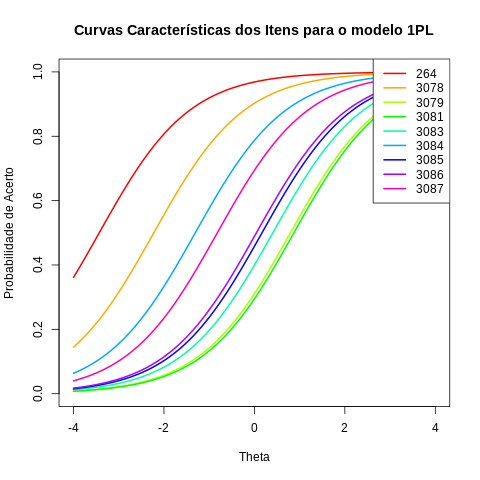
\includegraphics[width=0.32\textwidth, trim=10mm 16mm 0 2cm, clip]{ApeB_plot_1pl_ICC.png}
    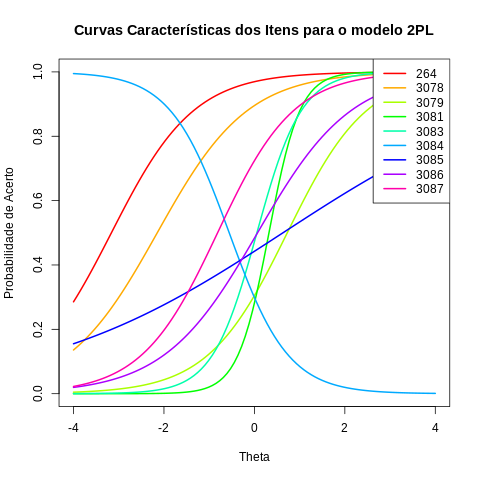
\includegraphics[width=0.32\textwidth, trim=10mm 16mm 0 2cm, clip]{ApeB_plot_2pl_ICC.png}
    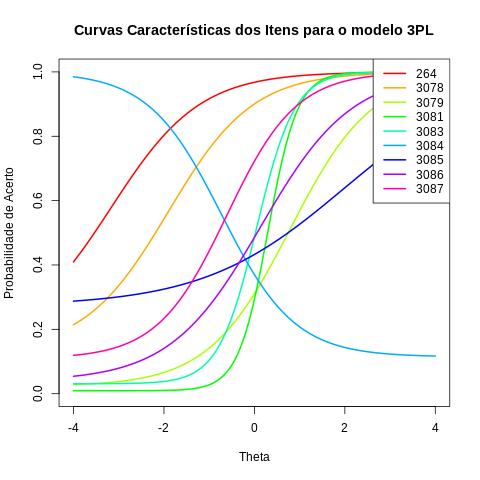
\includegraphics[width=0.32\textwidth, trim=10mm 16mm 0 2cm, clip]{ApeB_plot_3pl_ICC.png}
    \caption{Curvas Características dos Itens nos modelos 1PL (esquerda), 2PL (centro) e 3PL (direita).}
    \label{fig:ApeB_plot_ALL_ICC}
    \end{figure}


\subsubsection{Curvas de Informação ao Item}\label{sec:apeB_cci}

A Figura \ref{fig:ApeB_plot_CII} apresenta as Curvas de Informação ao Item (CII) para os modelos 2PL e 3PL, respectivamente, utilizando a função \verb|mirt()| do pacote R chamado \verb|mirt|. Nos modelos 2PL e 3PL, os itens 3081 e 3083  apresentam picos altos de informação, sugerindo que esses itens fornecem uma quantidade substancial de informação sobre a habilidade dos indivíduos em uma região específica do traço latente. Esse comportamento é típico de itens com alta capacidade discriminativa, porém, pode indicar que esses itens são mais adequados para diferenciar indivíduos com habilidades próximas ao ponto de máxima informação do item, sendo menos eficientes em distinguir indivíduos com habilidades distantes desse ponto.

\begin{figure}[!ht]
\centering
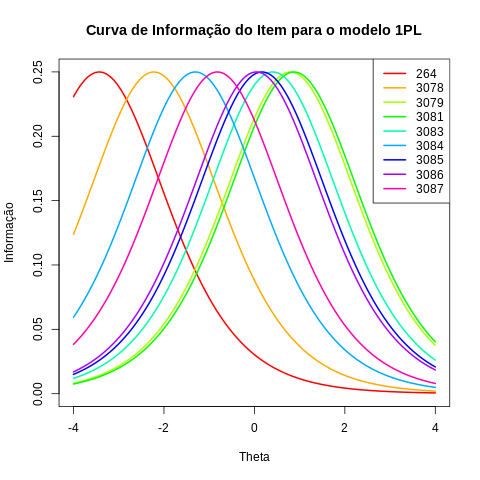
\includegraphics[width=0.32\textwidth, trim=10mm 16mm 0 2cm, clip]{ApeB_plot_1pl_CII.png}
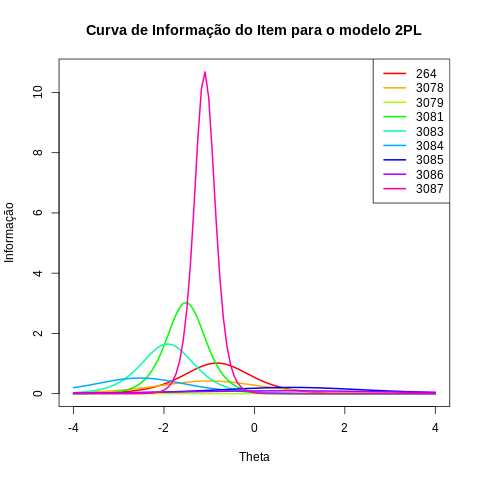
\includegraphics[width=0.32\textwidth, trim=10mm 16mm 0 2cm, clip]{ApeB_plot_2pl_CII.png}
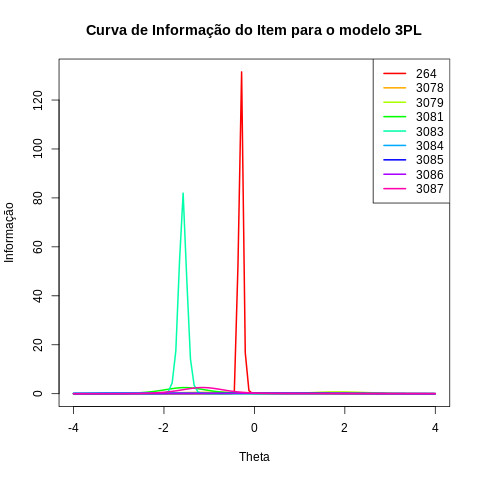
\includegraphics[width=0.32\textwidth, trim=10mm 16mm 0 2cm, clip]{ApeB_plot_3pl_CII.png}
\caption{Curvas de Informação ao Item nos modelos 1PL (esquerda), 2PL (centro) e 3PL (direita).}
\label{fig:ApeB_plot_CII}
\end{figure}

\subsubsection{Curvas de Informação do Teste}\label{sec:apeB_cit}

A Figura \ref{fig:ApeB_plot_TIC} apresenta as Curvas de Informação do Teste (CIT) para os modelos 1PL, 2PL e 3PL. Observa-se que as CITs nestes modelos atinge picos próximos da habilidade $\theta = 0$, com valores máximos de informação entre 1 e 5. As CITs se concentram na região entre $\theta = -2$ e $\theta = 2$, indicando que o teste possui maior precisão de medição em torno dessa faixa de habilidade. 

\begin{figure}[!ht]
    \centering
    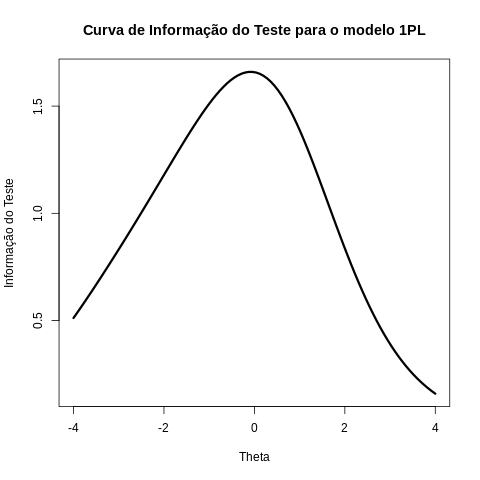
\includegraphics[width=0.32\textwidth, trim=10mm 16mm 0 2cm, clip]{ApeB_plot_1pl_TIC.png}
    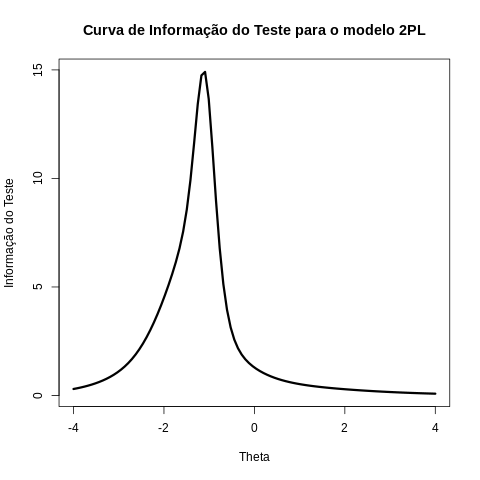
\includegraphics[width=0.32\textwidth, trim=10mm 16mm 0 2cm, clip]{ApeB_plot_2pl_TIC.png}
    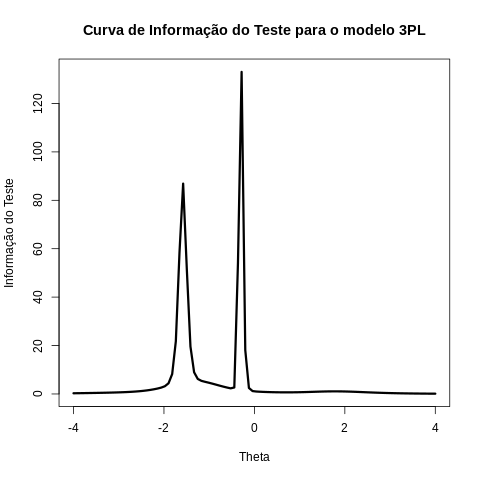
\includegraphics[width=0.32\textwidth, trim=10mm 16mm 0 2cm, clip]{ApeB_plot_3pl_TIC.png}
    \caption{Curvas de Informação do Teste nos modelos 1PL (esquerda), 2PL (centro) e 3PL (direita).}
    \label{fig:ApeB_plot_TIC}
    \end{figure}

\subsubsection{Curvas de Informação vs Erro Padrão do Teste}\label{sec:apeB_TIC_SE}

A Figura \ref{fig:ApeB_plot_TIC_SE} exibe o TIC e SEM para os modelos 1PL, 2PL e 3PL. A análise comparativa desses modelos revela características interessantes, com máxima informação em torno de $\theta = 0$, além de interseções entre as curvas do TIC e SEM perto de -2 e 2. Além disso, o TIC em forma de sino apresenta quedas mais acentuadas para 2PL e 3PL à medida que se afasta de $\theta = 0$, enquanto o SEM aumenta em torno do ponto mínimo em $\theta = 0$, indicando maior precisão de medição perto do ponto mínimo e menor precisão em traços latentes extremos.

%Quando há uma interseção entre o TIC e o SEM, isso indica uma melhor adequação na medição de habilidades dentro desse intervalo de interseção \cite{?}.

\begin{figure}[!ht]
    \centering
    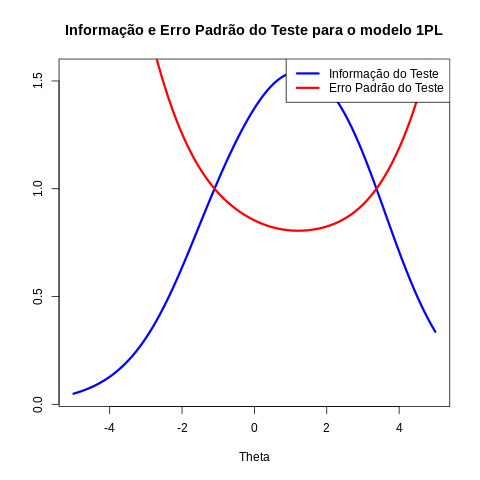
\includegraphics[width=0.32\textwidth, trim=10mm 16mm 0 2cm, clip]{ApeB_plot_1pl_TIC_SE_ex2.png}
    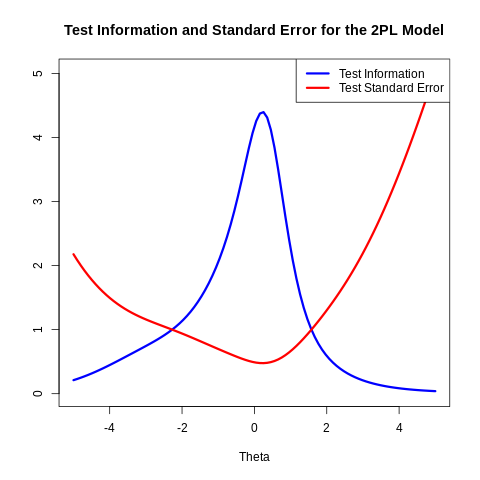
\includegraphics[width=0.32\textwidth, trim=10mm 16mm 0 2cm, clip]{ApeB_plot_2pl_TIC_SE_ex2.png} 
    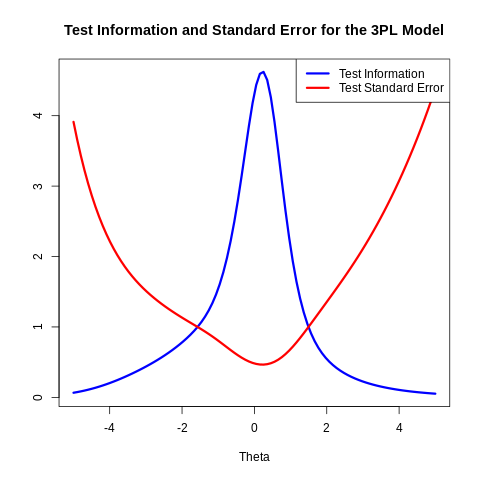
\includegraphics[width=0.32\textwidth, trim=10mm 16mm 0 2cm, clip]{ApeB_plot_3pl_TIC_SE_ex2.png}     
    \caption{Curvas de Informação vs Erro Padrão do Teste nos modelos 1PL (esquerda), 2PL (centro) e 3PL (direita).}
    \label{fig:ApeB_plot_TIC_SE}
    \end{figure}


  
\section{Questionário avaliativo}

Conforme detalhado no Apêndice \ref{ch:apendice} -- \nameref{ch:apendice}, houve um total de 72 estudantes matriculados em duas turmas: A, com 38 estudantes, e B, com 34 estudantes. A taxa de reprovação na turma A foi de 55,26\%, enquanto na turma B foi de 32,35\%. Isso resultou em 17 estudantes aprovados na turma A e 23 na turma B, totalizando 40 estudantes aprovados no curso.
\
Após a semana 11 do curso, um questionário foi disponibilizado para todos os estudantes matriculados; entretanto, apenas 17 deles (23.6\%) responderam, sendo 6 na turma A e 11 na turma B. 

\subsection{Questões aplicadas}

A seguir, são apresentadas as questões do questionário e um resumo das respostas dos estudantes. Foi utilizada a escala Likert com os seguintes valores: 1 - Discordo totalmente; 2 - Discordo; 3 - Indiferente; 4 - Concordo; 5 - Concordo totalmente.

\subsubsection{Questões gerais}

Esta seção aborda questões gerais relacionadas ao conhecimento prévio dos estudantes sobre linguagens de programação, suas percepções sobre o aprendizado e expectativas em relação à disciplina. A Figura \ref{fig:fig_col_General_questions} mostra BoxPlot \cite{tukey1977box} das respostas dos estudantes a essas questões.

É possível destacar que, nas questões Q3 e Q4, com média de 4,3, os estudantes demonstraram uma alta percepção da importância de conhecer linguagens de programação, mesmo com a presença de dois \textit{outliers}.

\begin{enumerate}[label=\textbf{Q\arabic*.}, itemsep=0pt, parsep=0pt, topsep=0pt, leftmargin=*, before=\ttfamily, after=\normalfont]
    \fontsize{9}{11}\selectfont
    \item O meu conhecimento de Linguagem de Programação (LP) ANTES de cursar PI já era muito bom;
    \item O meu conhecimento de LP APÓS o final de PI melhorou muito;
    \item Conhecer LPs pode ajudar na minha ATUAÇÃO ACADÊMICA, em OUTRAS DISCIPLINAS;
    \item Conhecer LPs pode ajudar na minha ATUAÇÃO PROFISSIONAL;
    \item Aula PRESENCIAL na TEORIA (no Laboratório) é melhor para o aprendizado;
    \item Aula PRESENCIAL na PRÁTICA (no Laboratório) é melhor para o aprendizado.
\end{enumerate}

\begin{figure}[!ht]
    \centering
    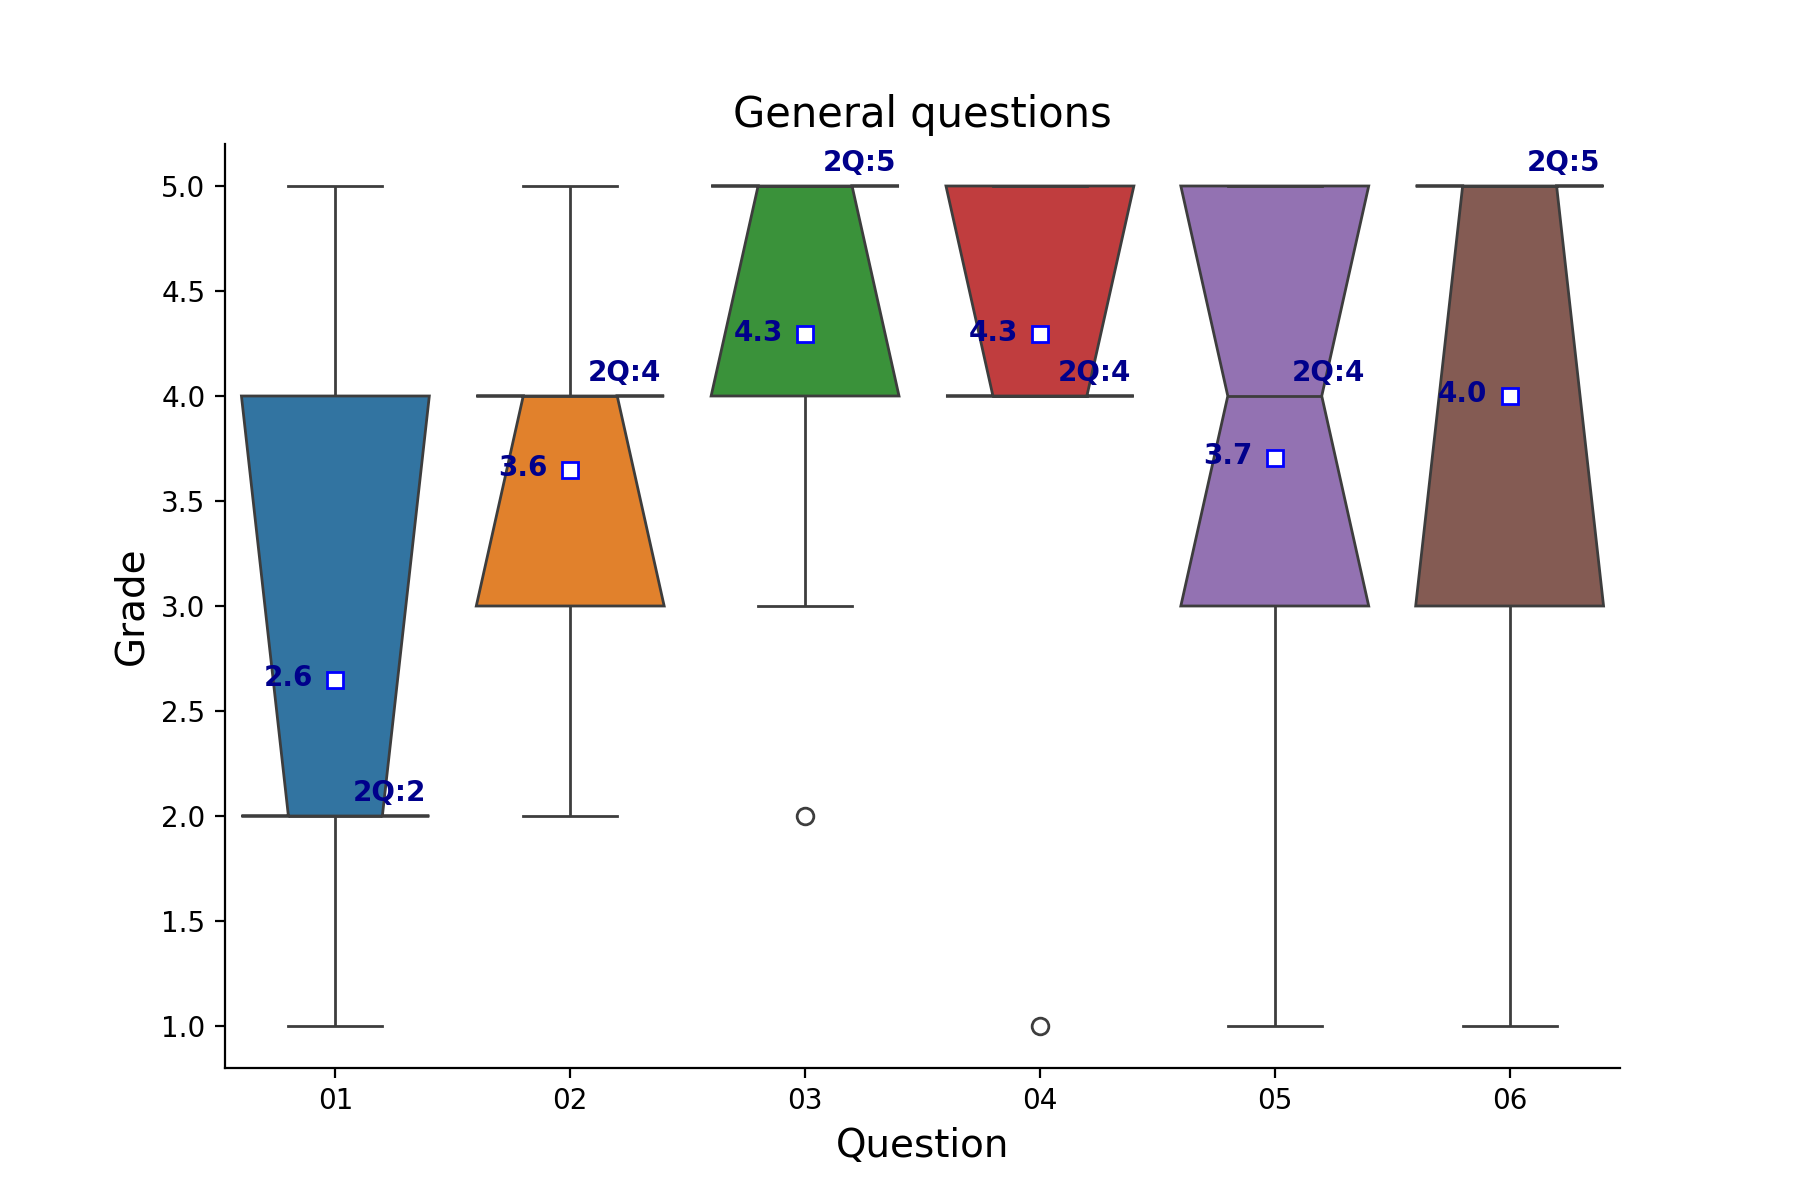
\includegraphics[width=0.7\textwidth]{fig_col_General_questions.png}
     \caption{Questionário com questões gerais.}
  \label{fig:fig_col_General_questions}
\end{figure}

\subsubsection{Questões sobre material de ensino}

A Figura \ref{fig:fig_col_Questions_about_Teaching_Material} apresenta questões relacionadas ao material didático utilizado na disciplina, incluindo a importância da diversidade de linguagens de programação e o \textit{feedback} sobre o material oferecido, com destaque para a Q8 sobre o uso do Colab, que recebeu uma média de 4.3. Segue a descrição completa dessas questões:

\begin{enumerate}[label=\textbf{Q\arabic*.}, itemsep=0pt, parsep=0pt, topsep=0pt, leftmargin=*, before=\ttfamily, after=\normalfont]
    \fontsize{9}{11}\selectfont
    \setcounter{enumi}{6} % Define o contador para iniciar em 07
    \item Acho importante que MATERIAL DIDÁTICO seja oferecido em várias LPs, a escolha do estudante;
    \item É importante o uso do COLAB como MATERIAL DIDÁTICO em PI;
    \item Acho importante os vídeos das aulas sobre o COLAB disponíveis em \url{https://sites.google.com/site/fzampirolli/pi-2024-1};
    \item Eu recomendaria aos colegas essa disciplina, ofertando MATERIAL DIDÁTICO com várias LPs;
    \item O MATERIAL DIDÁTICO com várias LPs que foi oferecido na minha turma é muito bom.
\end{enumerate}

\begin{figure}[!ht]
    \centering
    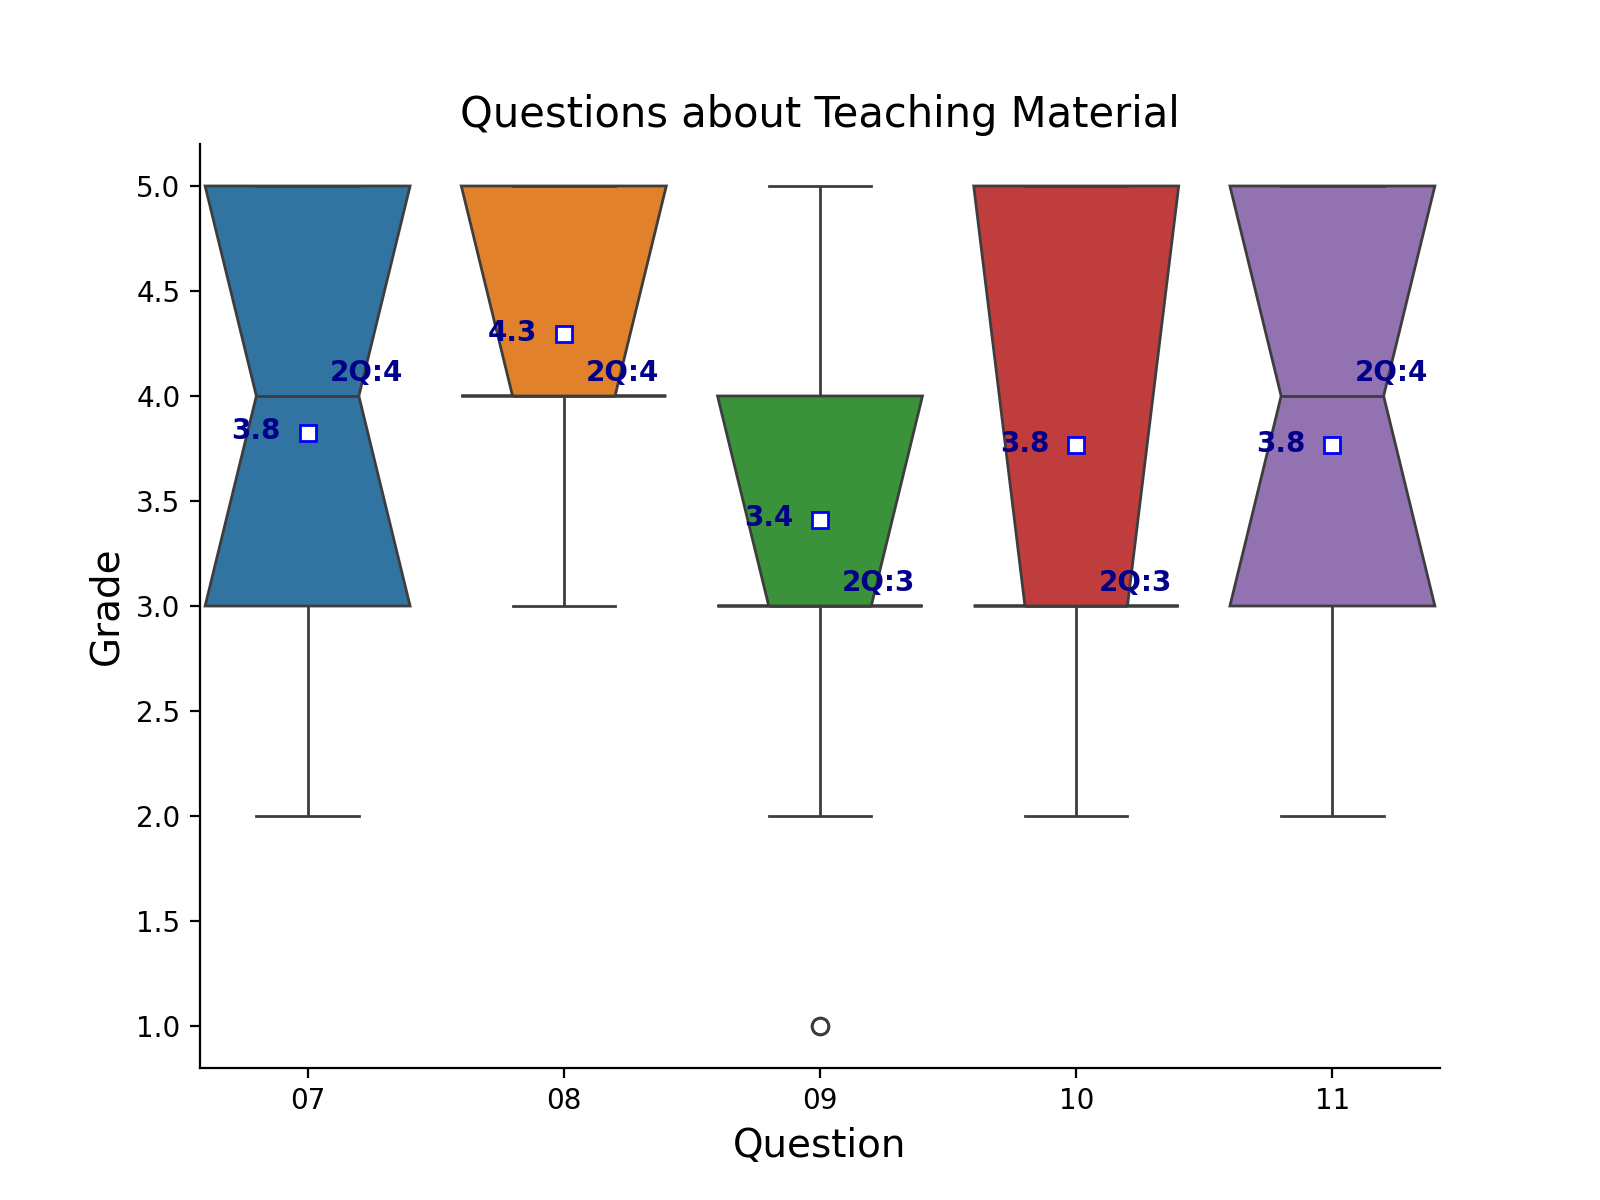
\includegraphics[width=0.7\textwidth]{fig_col_Questions_about_Teaching_Material.png}
     \caption{Questionário com questões sobre material de ensino.}
  \label{fig:fig_col_Questions_about_Teaching_Material}
\end{figure}


\subsubsection{Questões sobre avaliações}

Na Figura \ref{fig:fig_col_Questions_about_Assessment}, são abordadas questões sobre as atividades e avaliações realizadas na disciplina, incluindo a opinião dos estudantes sobre o uso de plataformas de avaliação \textit{online}. O destaque nessa parte foi que a média em todos os itens ficou próxima de 4. Segue a descrição completa dessas questões:

\begin{enumerate}[label=\textbf{Q\arabic*.}, itemsep=0pt, parsep=0pt, topsep=0pt, leftmargin=*, before=\ttfamily, after=\normalfont]
    \fontsize{9}{11}\selectfont
    \setcounter{enumi}{11} % Define o contador para iniciar em 12
    \item Acho importante oferecer ATIVIDADES em várias LPs, a escolha do estudante;
    \item É muito interessante o uso do Moodle+VPL nas ATIVIDADES (EPs e Provas) com correção automática e feedback imediato;
    \item A AVALIAÇÃO INDIVIDUAL ajuda a diminuir plágios, logo ajuda no aprendizado;
    \item Eu recomendaria aos meus colegas essa disciplina com a oferta de EPs com várias LPs;
    \item Os EPs com várias LPs que foram oferecidos na minha turma são muito bons.
\end{enumerate}

\begin{figure}[!ht]
    \centering
    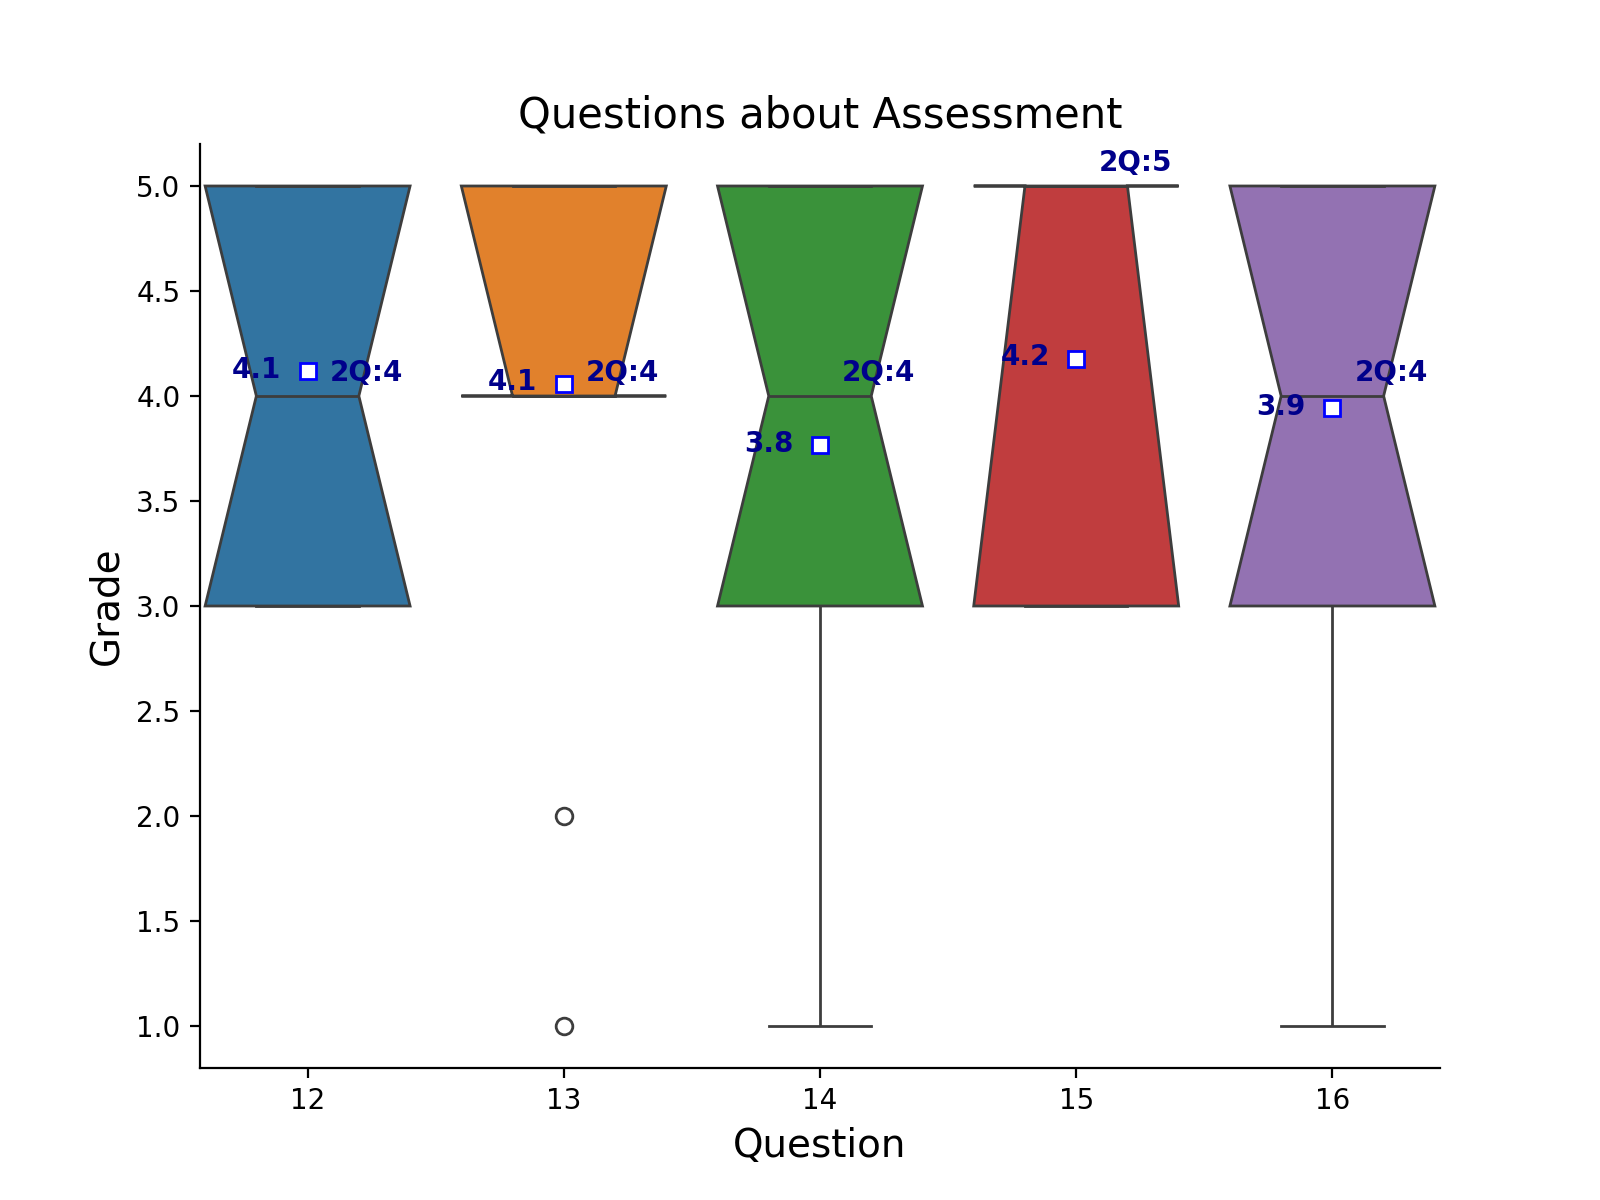
\includegraphics[width=0.7\textwidth]{fig_col_Questions_about_Assessment.png}
     \caption{Questionário com questões sobre avaliações.}
  \label{fig:fig_col_Questions_about_Assessment}
\end{figure}

\subsubsection{Questões sobre teste adaptativo}

Por fim, na Figura \ref{fig:fig_col_Questions_about_Adaptative_Questions}, são exploradas as percepções dos estudantes sobre os testes adaptativos, incluindo sua utilidade, desafios e influência nos hábitos de estudo. As respostas indicam que os estudantes consideram os Testes Semanais Individuais importantes (Q17 com média de 3.8), relatam uma melhora na confiança e compreensão dos conceitos de lógica de programação (Q18 com média de 3.5), percebem os testes adaptativos como desafiadores (Q19 com média de 4.0), afirmam que os testes adaptativos influenciaram seus hábitos de estudo (Q20 com média de 3.3) e concordam que os testes adaptativos proporcionaram desafios personalizados que atendiam às suas necessidades de aprendizagem (Q21 com média de 3.4). Destaca-se que as médias das respostas variaram entre 3.3 e 4.0, refletindo uma avaliação positiva geral em relação a esses aspectos. 

\begin{enumerate}[label=\textbf{Q\arabic*.}, itemsep=0pt, parsep=0pt, topsep=0pt, leftmargin=*, before=\ttfamily, after=\normalfont]
    \fontsize{9}{11}\selectfont
    \setcounter{enumi}{16} % Define o contador para iniciar em 17
    \item Acho importante os Testes Semanal Individual;
    \item Houve melhora na confiança e compreensão dos conceitos de lógica de programação;
    \item Os testes adaptativos foram desafiadores;
    \item Os testes adaptativos influenciaram nos hábitos de estudo;
    \item Os testes adaptativos proporcionaram desafios personalizados que atendiam; às necessidades de a\-prendizagem.
\end{enumerate}

\begin{figure}[!ht]
    \centering
    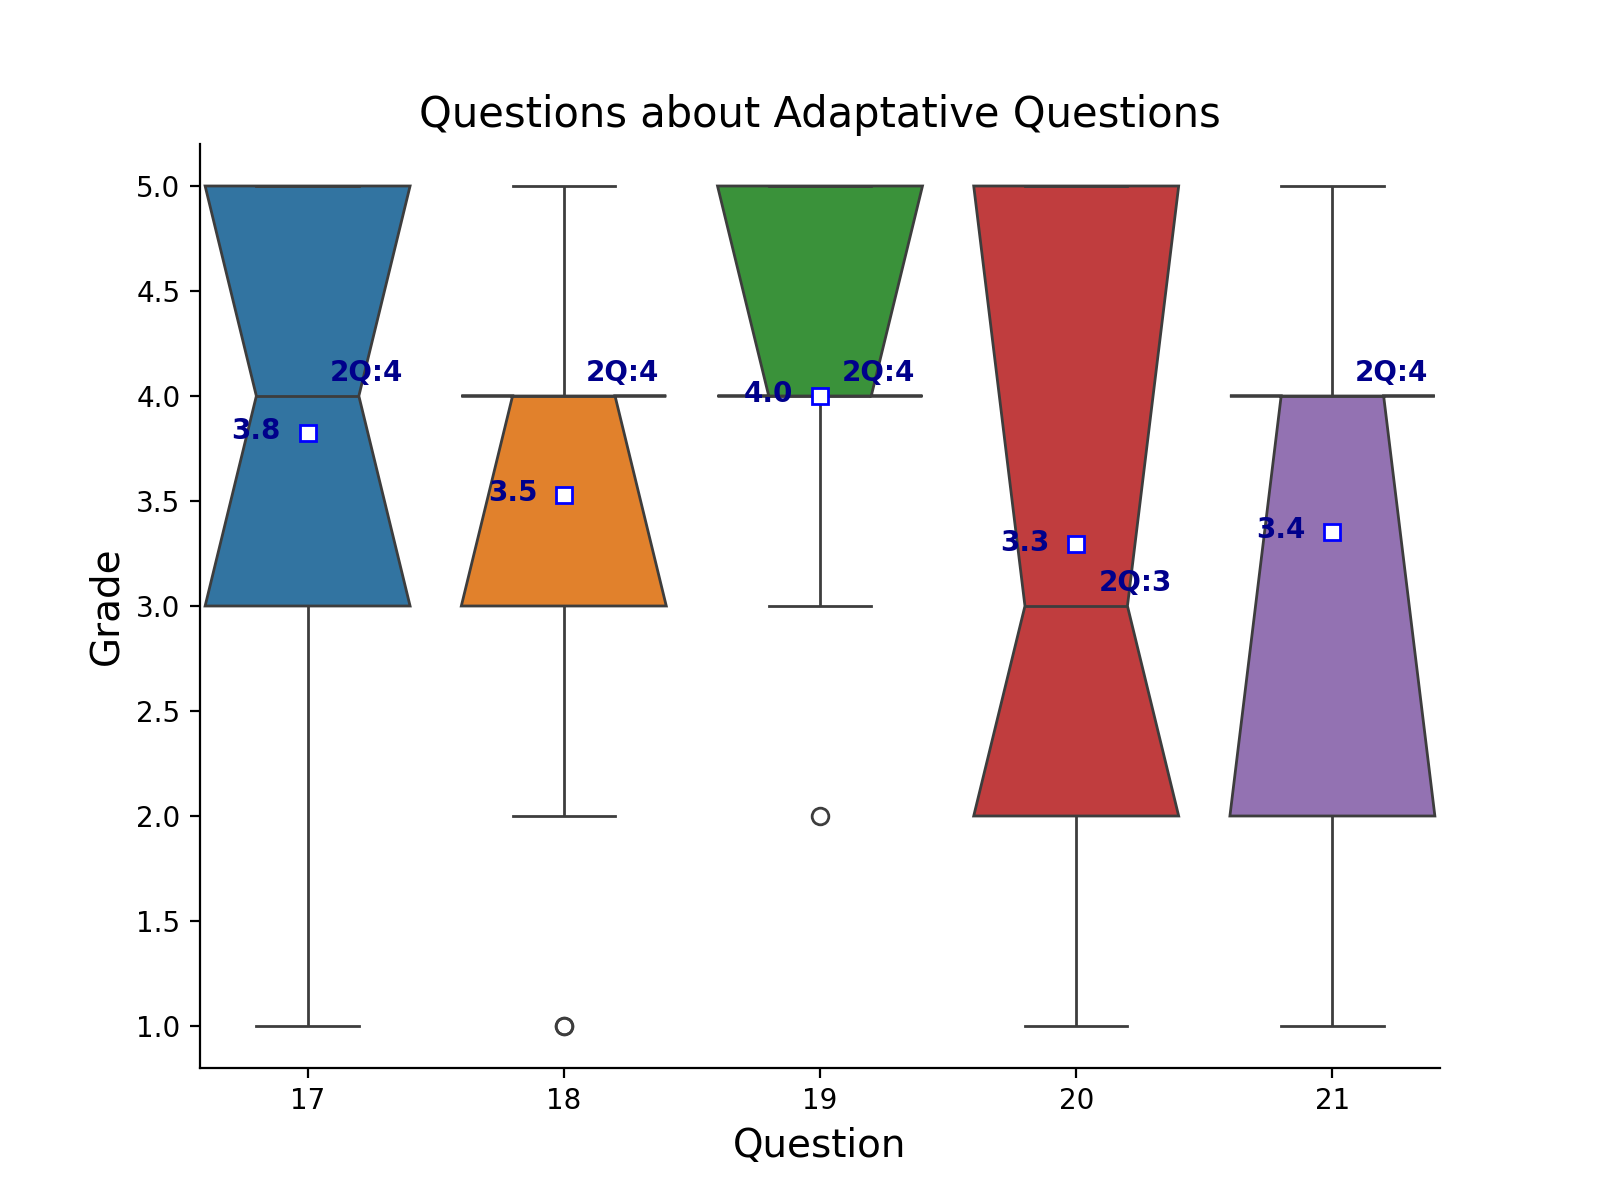
\includegraphics[width=0.7\textwidth]{fig_col_Questions_about_Adaptative_Questions.png}
     \caption{Questionário com questões sobre teste adaptativo.}
  \label{fig:fig_col_Questions_about_Adaptative_Questions}
\end{figure}

A Figura \ref{fig:fig_col_Questions_about_Adaptative_Questions-17} apresenta diversas medidas estatísticas da questão Q17, que não foram mostradas nas figuras anteriores, utilizando o modelo \textit{Violin Plots} \cite{hintze1998violin}.

\begin{figure}[!ht]
    \centering
    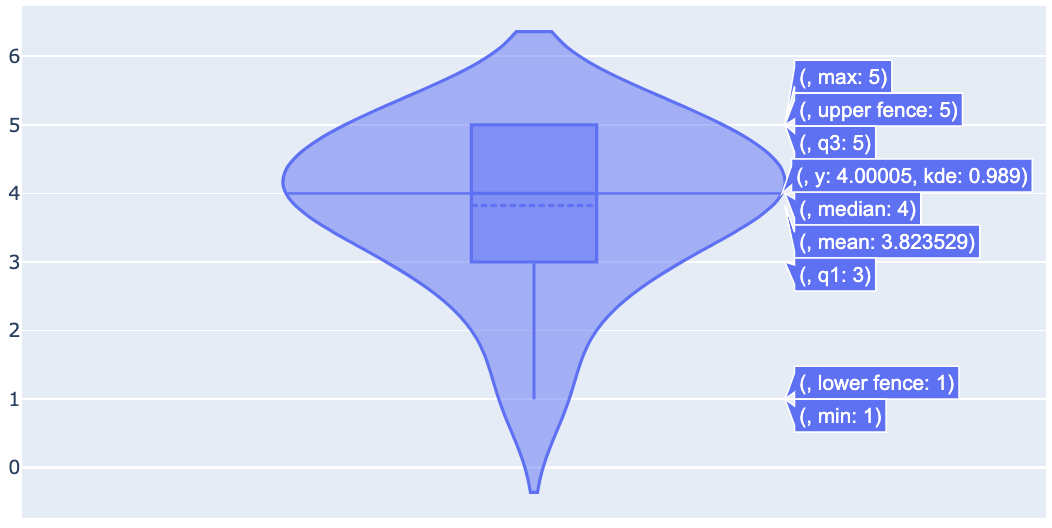
\includegraphics[width=0.7\textwidth]{fig_col_Questions_about_Adaptative_Questions-17.png}
    %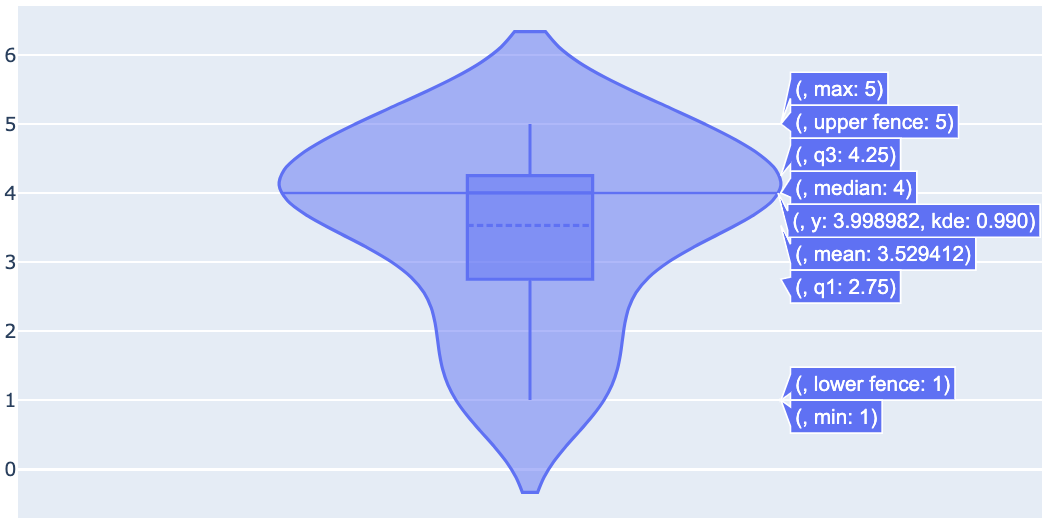
\includegraphics[width=0.49\textwidth]{fig_col_Questions_about_Adaptative_Questions-18.png}
     \caption{Destaque para a Q17. Acho importante os Testes Semanal Individual.}
  \label{fig:fig_col_Questions_about_Adaptative_Questions-17}
\end{figure}

\subsection{Análise estatística dos resultados}

Complementando os resultados da análise descritiva apresentada na seção anterior, a Tabela \ref{tab:estatisticas} apresenta os resultados de um teste estatístico realizado em um conjunto de dados com as respostas de 17 estudantes às 20 questões de múltipla escolha e duas questões abertas. O objetivo do teste é investigar se a média das respostas dos estudantes para cada questão é significativamente maior do que 3, indicando um impacto positivo da metodologia no aprendizado dos participantes. Para essa análise, foi utilizado o teste t de uma amostra para uma média (\(\bar{x}\)), com um nível de significância de 5\% \cite{lowry2014concepts}.
\
As hipóteses para o teste foram definidas da seguinte maneira:

\textbf{\( H_0 \)}: A metodologia teve um efeito neutro no aprendizado dos estudantes, ou seja, \( \bar{x} \leq 3 \).

\textbf{\( H_1 \)}: A metodologia teve um impacto positivo no aprendizado dos estudantes, ou seja, \( \bar{x} > 3 \).

Para decidir se rejeita ou não a hipótese nula (\( H_0 \)), é comparado o p-Value resultante do teste t com o nível de significância. Se o p-Value for menor que o nível de significância (0.05), então rejeita-se a hipótese nula. Isso indica que há evidências estatísticas de que a média das respostas é significativamente maior do que 3. Na última coluna da tabela, um ``X'' denota a não rejeição da hipótese nula. Ou seja, as questões marcadas não apresentam significância estatística para afirmar que a metodologia teve um impacto positivo no aprendizado.

A tabela também fornece outras estatísticas relevantes, como média, mediana, p-Value, Efeito e Poder. O p-Value é a probabilidade de obter um resultado tão extremo quanto (ou mais extremo do que) o observado, assumindo que a hipótese nula é verdadeira. O Efeito mede a magnitude da diferença entre a média observada e o valor de referência (3 neste caso), expresso em unidades de desvio padrão. O Poder do teste é a probabilidade de rejeitar a hipótese nula quando ela é falsa, ou seja, a capacidade do teste de detectar um efeito significativo, se houver um.

É importante lembrar que, embora um p-Value menor que o nível de significância indique que a média das respostas é significativamente maior do que 3, isso não implica necessariamente que a metodologia teve um impacto positivo no aprendizado dos estudantes. Pode haver outros fatores não considerados no estudo que também podem influenciar as respostas dos estudantes. Além disso, o poder do teste depende do tamanho do efeito e do tamanho da amostra. Portanto, um alto poder do teste não garante que a hipótese nula será rejeitada, mas sim que o teste tem uma alta probabilidade de detectar um efeito significativo, se houver um.

Os resultados da análise indicam que a metodologia de ensino adotada teve um efeito positivo no aprendizado dos estudantes. A maioria das questões do questionário apresentou significância estatística, com médias de respostas acima de 3. Isso sugere que os estudantes que participaram do estudo consideraram a metodologia útil e eficaz para o seu aprendizado.

Embora esses resultados sejam promissores, é importante ressaltar que novas pesquisas são necessárias para confirmar a efetividade da metodologia em larga escala. Estudos futuros, com amostras maiores e mais diversificadas, incluindo grupos de teste e controle, permitiriam análises mais robustas e generalizações mais confiáveis sobre o impacto da metodologia no aprendizado de estudantes em diferentes contextos.

\begin{table}[!ht]
    \centering
    \caption{Tabela com os resultados estatísticos}
    \label{tab:estatisticas}
    \rowcolors{2}{gray!25}{white}\footnotesize
    \begin{tabular}{|c|c|c|c|c|c|c|}
        \hline
        \cellcolor{green!25} \textbf{Questão} & \cellcolor{green!25} \textbf{Média} & \cellcolor{green!25} \textbf{Mediana} & \cellcolor{green!25} \textbf{p-Value} & \cellcolor{green!25} \textbf{Efeito} & \cellcolor{green!25} \textbf{Poder} & \cellcolor{green!25} \textbf{H0} \\
        \hline
        Q1 & 2.65 & 2.0 & 0.29 & -0.27 & 1.07 & X \\
        Q2 & 3.65 & 4.0 & 0.01 & 0.69 & 0.82 &  \\
        Q3 & 4.29 & 5.0 & 0.00 & 1.41 & 0.64 &  \\
        Q4 & 4.29 & 4.0 & 0.00 & 1.31 & 0.66 &  \\
        Q5 & 3.71 & 4.0 & 0.05 & 0.52 & 0.87 &  \\
        Q6 & 4.00 & 5.0 & 0.01 & 0.69 & 0.82 &  \\
        Q7 & 3.82 & 4.0 & 0.00 & 0.87 & 0.78 &  \\
        Q8 & 4.29 & 4.0 & 0.00 & 1.68 & 0.57 &  \\
        Q9 & 3.41 & 3.0 & 0.20 & 0.32 & 0.92 & X \\
        Q10 & 3.76 & 3.0 & 0.01 & 0.74 & 0.81 &  \\
        Q11 & 3.76 & 4.0 & 0.01 & 0.67 & 0.83 &  \\
        Q12 & 4.12 & 4.0 & 0.00 & 1.30 & 0.66 &  \\
        Q13 & 4.06 & 4.0 & 0.00 & 0.97 & 0.75 &  \\
        Q14 & 3.76 & 4.0 & 0.02 & 0.61 & 0.84 &  \\
        Q15 & 4.18 & 5.0 & 0.00 & 1.24 & 0.68 &  \\
        Q16 & 3.94 & 4.0 & 0.01 & 0.75 & 0.81 &  \\
        Q17 & 3.82 & 4.0 & 0.01 & 0.73 & 0.81 &  \\
        Q18 & 3.53 & 4.0 & 0.12 & 0.40 & 0.90 & X \\
        Q19 & 4.00 & 4.0 & 0.00 & 1.15 & 0.70 &  \\
        Q20 & 3.29 & 3.0 & 0.40 & 0.21 & 0.95 & X \\
        Q21 & 3.35 & 4.0 & 0.30 & 0.26 & 0.93 & X \\
        \hline
    \end{tabular}\normalsize
\end{table}



\section{Considerações finais}

Este apêndice descreve uma experiência conduzida na disciplina de Processamento da Informação (CS1) na UFABC durante o primeiro quadrimestre de 2024, em duas turmas. O objetivo foi realizar seis testes, sendo cinco adaptativos ao longo do curso, como avaliações formativas, com peso de 5\% no conceito final, com bônus proporcional ao número de testes realizados. Os estudantes foram informados sobre esses testes adaptativos como uma estratégia motivacional aplicada na disciplina.

Os testes adaptativos utilizaram diferentes métodos, como SAT (\textit{Semi-Adaptive Testing}), WPC (\textit{Weighted Probability of Correctness}) e MLE (\textit{Maximum Likelihood Estimation}), com o objetivo de avaliar e acompanhar o progresso dos estudantes de forma personalizada. A análise dos resultados dos testes mostrou que os métodos adaptativos foram capazes de fornecer uma avaliação mais precisa e individualizada do aprendizado dos estudantes, permitindo que fossem propostos desafios personalizados de acordo com o nível de habilidade de cada um.

O questionário aplicado no final do curso indicou que a maioria dos estudantes considerou os testes adaptativos importantes, desafiadores e benéficos para o seu aprendizado, com impacto positivo na confiança e compreensão dos conceitos de lógica de programação. A análise estatística das respostas ao questionário revelou que a metodologia de ensino-aprendizagem-avaliação adotada, incluindo os testes adaptativos, teve um efeito positivo no aprendizado dos estudantes, com a maioria das questões apresentando significância estatística.

Embora os resultados sejam promissores, novos estudos com amostras maiores e mais diversificadas serão necessários para confirmar a efetividade da metodologia em larga escala e obter generalizações mais confiáveis. Esta experiência apresentou uma implementação bem-sucedida de testes adaptativos em uma disciplina introdutória de programação, com impactos positivos no aprendizado e engajamento dos estudantes, demonstrando ser uma estratégia motivacional eficaz que merece ser explorada em outros contextos educacionais.